%%%%%%%%%%%%%%%%%%%%%%%%%%%%%%%%%%%%%%%%%%%%%%%%%%%%%%%%%%%
% EPFL report package, main thesis file
% Goal: provide formatting for theses and project reports
% Author: Mathias Payer <mathias.payer@epfl.ch>
%
% To avoid any implication, this template is released into the
% public domain / CC0, whatever is most convenient for the author
% using this template.
%
%%%%%%%%%%%%%%%%%%%%%%%%%%%%%%%%%%%%%%%%%%%%%%%%%%%%%%%%%%%
\documentclass[a4paper,11pt,oneside]{report}
% Options: MScThesis, BScThesis, MScProject, BScProject
\usepackage[MScProject,lablogo]{EPFLreport}
\usepackage{xspace}

\title{JTAG support \\for Gecko5Education Board}
\author{Antoine Colson}
\supervisor{Prof. Ties Jan Henderikus Kluter}

\newcommand{\boardName}{Gecko5Education \xspace}

\begin{document}
\maketitle
% \makededication
% \makeacks

% \begin{abstract}
% The \sysname tool enables lateral decomposition of a multi-dimensional
% flux compensator along the timing and space axes.

% The abstract serves as an executive summary of your project.
% Your abstract should cover at least the following topics, 1-2 sentences for
% each: what area you are in, the problem you focus on, why existing work is
% insufficient, what the high-level intuition of your work is, maybe a neat
% design or implementation decision, and key results of your evaluation.
% \end{abstract}

% \begin{frenchabstract}
% For a doctoral thesis, you have to provide a French translation of the
% English abstract. For other projects this is optional.
% \end{frenchabstract}

\maketoc

%%%%%%%%%%%%%%%%%%%%%%
\chapter{Introduction}
%%%%%%%%%%%%%%%%%%%%%%

This project focuses on implementing and testing robust JTAG (Joint Test Action Group) communication and control for the \boardName board.
The primary objective is to develop low-level infrastructure that enables JTAG-based access to internal system components, providing a foundation for concrete and useful applications.

Several challenges were encountered in pursuing this goal.
First, the \boardName board was designed specifically for educational purposes at EPFL and lacks documentation, 
making its internal architecture, particularly in relation to JTAG communication, largely unexplored.
Second, no prior work has addressed JTAG support for this specific board; existing references mainly focus on other platforms or architectures.
Third, even the official Lattice documentation \cite{lattice_semiconductor_fpga_2020} for the specific FPGA used on the board is limited, 
offering only minimal guidance on implementing or extending JTAG functionality.
Finally, the onboard JTAG interface itself is minimalistic, 
providing only the core features mandated by the standard, with little support for custom extensions.

To address these challenges, the project was divided into two main milestones:

\begin{itemize}
    \item Establish basic communication via the JTAG interface and demonstrate control using the on-board RGB LEDs.
    \item Extend the JTAG interface to support memory access and peripheral control by enabling read and write operations to any component on the bus architecture.
\end{itemize}

In summary, this project aimed to transform the previously underutilized JTAG interface of the \boardName board into a powerful low-level communication path 
that can be used by EPFL students in future projects.
Both milestones were successfully completed: reliable communication with the board was achieved, 
and the interface was extended to provide full access to memory and peripherals.
As a result, software can now interact with the board through a high-level abstraction of the JTAG interface, 
hiding much of the underlying complexity.
The remainder of this report details the background of the project, the design and implementation of the involved components, and the evaluation of the enhanced JTAG interface.


%%%%%%%%%%%%%%%%%%%%
\chapter{Background}
%%%%%%%%%%%%%%%%%%%%

This chapter provides the foundational knowledge necessary to understand the design and implementation of the enhanced JTAG interface on the \boardName board.
It begins with an overview of the \boardName board itself, outlining its primary features.
Following this, essential FPGA concepts are introduced to clarify how the board’s programmable logic is utilized in the project.
Then, it explains the initial system architecture, which serves as the baseline for the JTAG enhancements.
Next, the chapter details the open-source toolchain employed throughout development, simulation, and debugging activities.
Finally, it presents an in-depth explanation of the JTAG protocol, its operation, signals, and finite state machine, which forms the core technology used throughout this project.

\section{The \boardName Board}
\label{sec:board}

The \boardName board is an FPGA development platform primarily  
used for teaching digital systems and computer architecture at EPFL \cite{noauthor_logisim-evolution/gecko5education_2025}.  
It is designed to give students hands-on experience and features  
a Lattice ECP5 FPGA at its core.  
The board also includes various peripherals suitable for system-on-chip experimentation,  
such as DRAM memory blocks, general-purpose I/Os (GPIOs) like push buttons and switches,  
an RGB LED matrix, and a UART interface for serial communication.  

Although the board provides a JTAG port through a USB-C connector,  
it was previously unused due to its minimal implementation and  
the availability of UART for communication.  

\section{FPGA Basics}

As mentioned in Section~\ref{sec:board}, the \boardName board is built around a Lattice ECP5 FPGA.
Unlike CPUs, which execute software instructions sequentially, FPGAs are reconfigurable hardware platforms used to implement custom digital logic circuits.
They are programmed using hardware description languages (HDLs); in this project, Verilog is used to describe the hardware’s structure and behavior.
The HDL code is then synthesized, placed, and routed to produce a bitstream, which is loaded into the FPGA to configure its logic.

In this project, the FPGA is used to extend an existing microcontroller-based architecture by adding components for JTAG support. 

\section{Initial System Architecture}
\label{sec:arch}

The default system architecture on the board is based on an OpenRISC microprocessor, implementing the OpenRISC 1000 ISA in a 5-stage pipelined configuration.
It is connected to other modules via a 32-bit shared bus.
The default setup includes a UART module, an SDRAM memory controller, a camera interface, and various GPIO components.

All modules are interconnected through the shared bus, which is designed to be easily extensible, an essential feature leveraged in the second milestone of this project.

In its default configuration, the system is capable of running arbitrary programs by communicating with the board through the UART interface.
Program output or debug feedback can be retrieved via UART or visually displayed by connecting a monitor to the board’s HDMI port.

The SDRAM is mapped to the beginning of the memory space at address \texttt{0x00000000} and provides 32MiB of storage.

For the first milestone, the JTAG interface was used only to control the RGB LEDs, which are directly mapped to GPIOs. Hence this architecture becomes relevant only for the second milestone,  
where the JTAG interface is extended to support memory and peripheral access.  

\section{Toolchain}
\label{sec:toolchain}

The project uses the open-source \texttt{oss-cad-suite} \cite{noauthor_yosyshq/oss-cad-suite-build_2025}, a comprehensive collection of tools for FPGA development.
Icarus Verilog is used for simulation, and GTKWave is employed for waveform visualization.
Yosys handles synthesis, while nextpnr-ecp5 performs placement and routing.
The bitstream is then generated using \texttt{ecppack} and loaded onto the FPGA using \texttt{openFPGALoader}.

Additionally, \texttt{OpenOCD} (Open On-Chip Debugger) \cite{noauthor_openocd-org/openocd_2025} is used  
to interact with the JTAG interface.  
It provides a telnet-accessible environment to send low-level JTAG commands,  
making it possible to control TAP state machine and directly drive input signals.  


\section{JTAG Protocol}
\label{sec:JTAG}

The JTAG protocol is the core focus of this project.  
Defined by the IEEE 1149.1 standard \cite{ieee1149_1_1990},  
JTAG (Joint Test Action Group) was introduced in the 1990s  
to facilitate testing and debugging of printed circuit boards.  
It uses boundary-scan techniques to check inter-chip connections  
without requiring physical access to individual pins.  

Today, JTAG is also widely used for in-system programming, secure provisioning,  
and system-level debugging in embedded systems.  

The interface includes four required signals and one optional:  

\begin{itemize}
    \item \textbf{TDI (Test Data In)} — Serial input line.  
    \item \textbf{TDO (Test Data Out)} — Serial output line.  
    \item \textbf{TCK (Test Clock)} — Synchronizes data shifting.  
    \item \textbf{TMS (Test Mode Select)} — Drives the JTAG finite state machine.  
    \item \textbf{TRST (Test Reset)} — Optional asynchronous reset line.  
\end{itemize}

JTAG communication is governed by the TAP (Test Access Port) controller,  
which operates as a finite state machine.  
Figure~\ref{fig:tap-fsm} illustrates the TAP state diagram as defined in the JTAG standard.

\begin{figure}
    \centering
    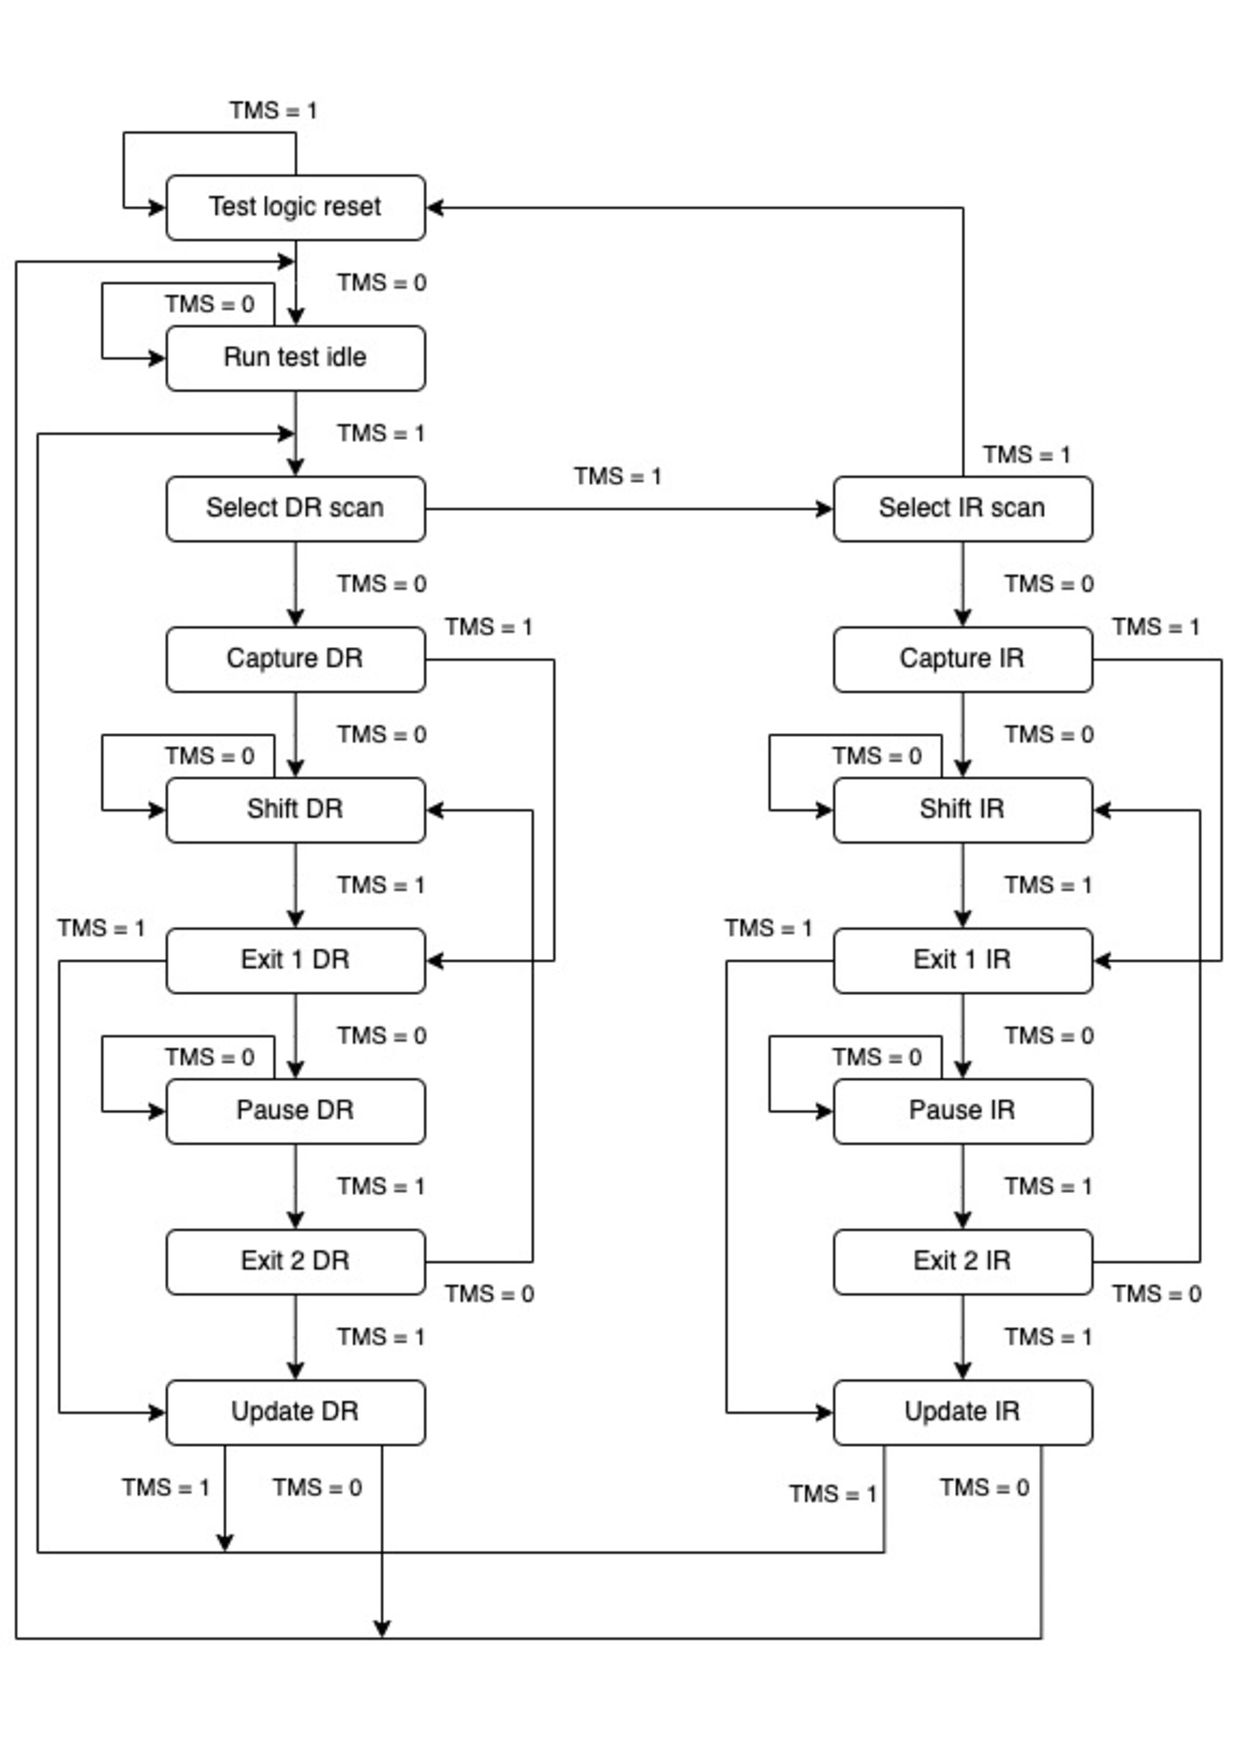
\includegraphics[width=0.6\textwidth]{figures/TAP_FSM.pdf} % or .png, .eps, etc.
    \caption{TAP controller finite state machine as defined by the IEEE 1149.1 standard.}
    \label{fig:tap-fsm}
\end{figure}

Key states include:  

\begin{itemize}
    \item \textbf{Test-Logic Reset} — Resets the TAP controller.  
    \item \textbf{Run-Test/Idle} — Wait state for idle periods.  

    \item \textbf{Capture-IR} — Loads the currently used instruction value into the instruction register to prepare for shfting out.
    \item \textbf{Shift-IR} — Serially shifts bits into the instruction register via TDI, while shifting out old bits via TDO.
    \item \textbf{Update-IR} — Transfers the newly shifted instruction into the active instruction register, making it effective.
    
    \item \textbf{Capture-DR} — Captures current data from the selected data register.
    \item \textbf{Shift-DR} — Serially shifts data through the data register, enabling read/write access via TDI/TDO.
    \item \textbf{Update-DR} — Loads the newly shifted data into the active data register, completing the data operation.
\end{itemize}

The TAP state transitions are determined by the TMS input on rising edges of TCK.  
By controlling TMS, TDI, and TCK, users can navigate the state machine,  
shift in instructions, and exchange data.  

Because JTAG relies on shift registers, it supports bidirectional communication:  
data can be shifted in via TDI and read out via TDO simultaneously.  
In this project, this mechanism is used to control LEDs  
and access memory and peripheral modules on the \boardName board.  
Hence understanding the JTAG protocol and its operation is crucial for the design and implementation of the JTAG interface.


%%%%%%%%%%%%%%%%
\chapter{JTAG Interface Designs}
%%%%%%%%%%%%%%%%

This chapter details the design decisions and implementation steps taken to enable JTAG-based control on the \boardName board.
We begin by introducing the existing JTAGG interface, which forms the foundational component of the project.
Next, we describe the implementation for Milestone 1, which focuses on using the JTAG interface to control the RGB LEDs through GPIOs.
Finally, we present the design and functionality introduced in Milestone 2, where the JTAG interface is extended to support memory-mapped access to system peripherals.

\section{JTAG Interface Block: JTAGG}

On the \boardName board, the JTAG interface is implemented using a Lattice ECP5 FPGA \cite{lattice_semiconductor_fpga_2020}.
This FPGA includes a built-in JTAG interface module called \texttt{JTAGG} that can be instantiated and used in the design.
This module handles the JTAG protocol and provides the necessary signals for communication,
respecting the standard JTAG definition explained in Section~\ref{sec:JTAG}.

The \texttt{JTAGG} module provides the standard ports \texttt{TDI}, \texttt{TDO}, \texttt{TCK}, and \texttt{TMS},
and is controlled by a TAP controller as described in Section~\ref{sec:JTAG}.
Additionally, it provides signals for two custom develloper designed instructions that become active when the values
\texttt{0x32} and \texttt{0x38} are shifted into the instruction register,
corresponding to \texttt{ER1} and \texttt{ER2}, respectively.
Unfortunately, the Lattice documentation provides limited details on this module.
However, Tom Verbeure has implemented a concrete and detailed version of it in a GitHub repository \cite{verbeure_tomverbeure/ecp5_jtag_2025},
which I used both to understand the \texttt{JTAGG} module and to test my design through simulation.

This module exposes a set of pins that can be used to implement these two custom instructions.
The corresponding block diagram is shown in Figure~\ref{fig:jtagg_block}.
Below is a summary of the signals provided by the \texttt{JTAGG} module.
All these signals are one bit wide.

\begin{figure}
    \centering
    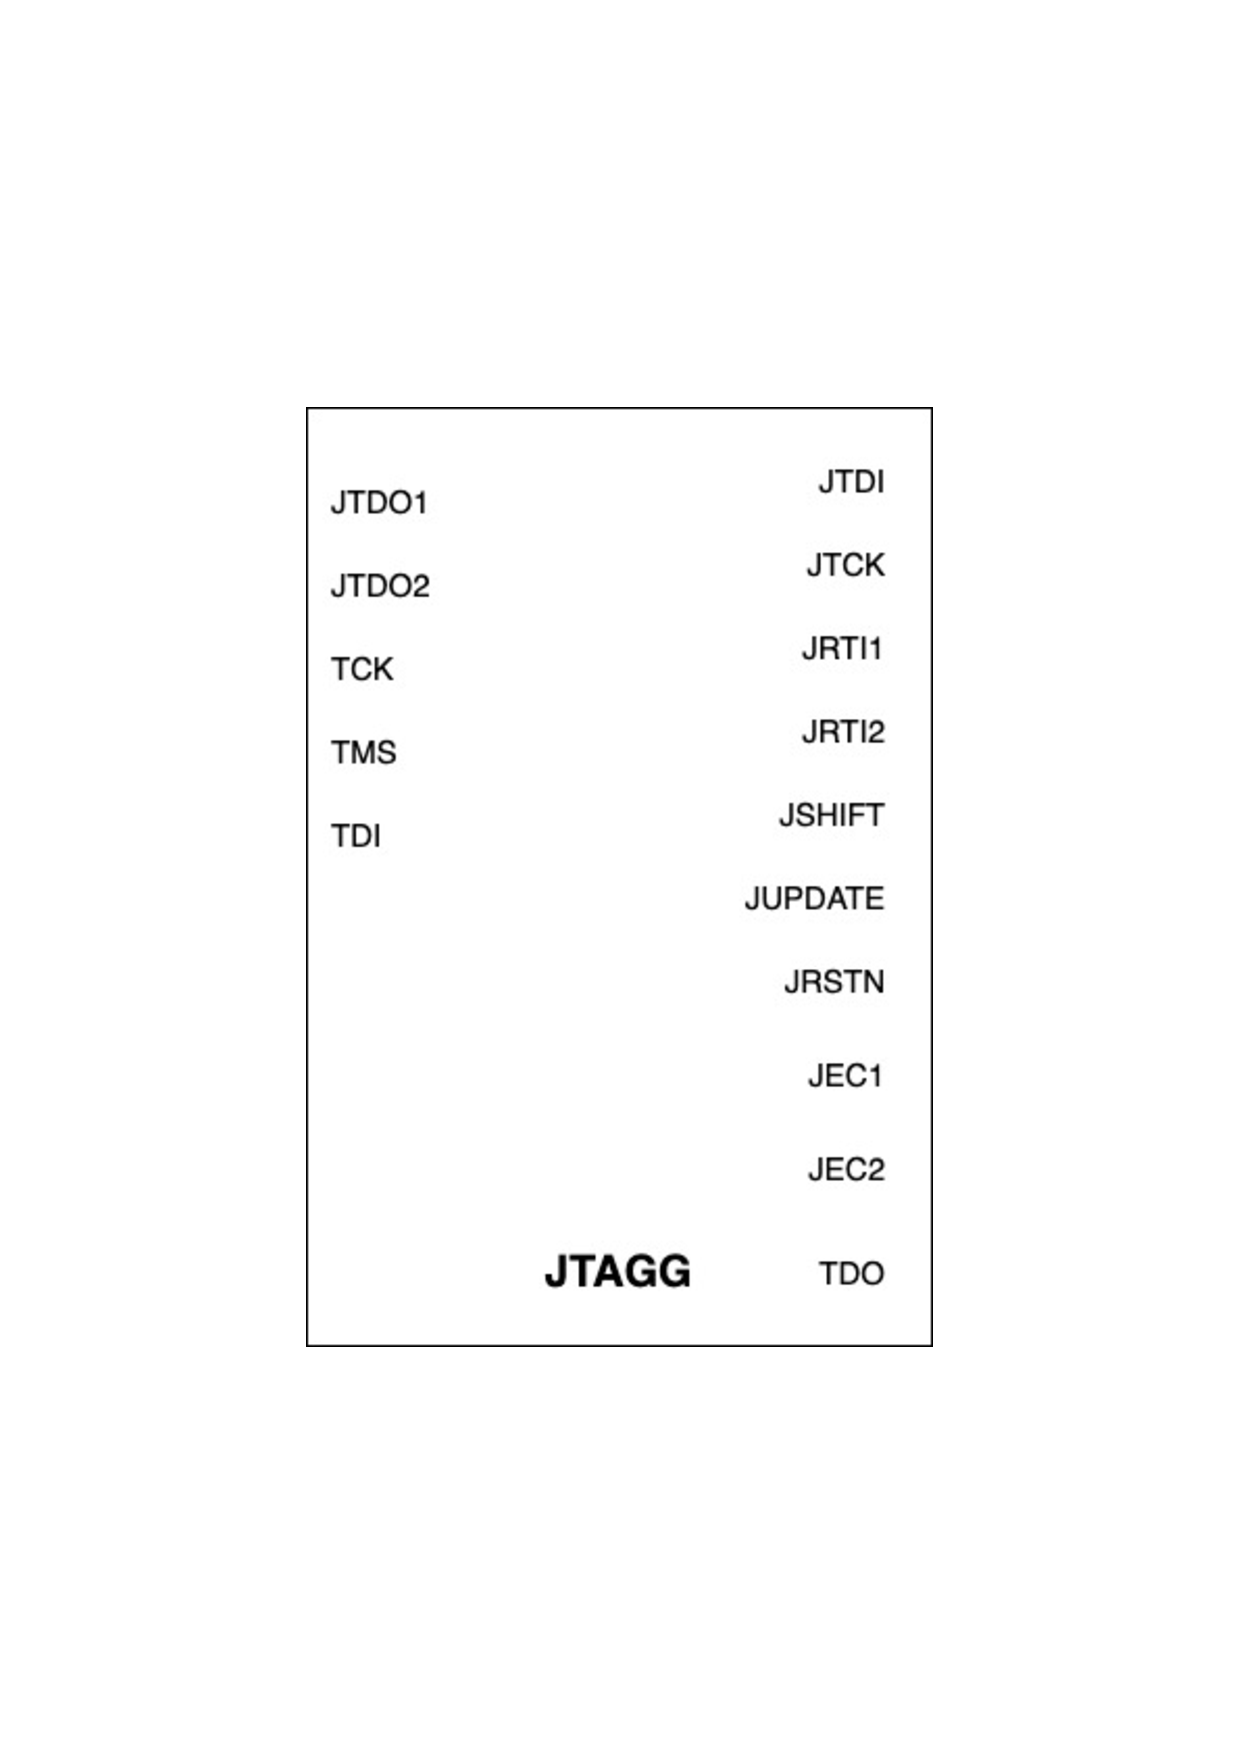
\includegraphics[width=0.9\linewidth]{figures/jtagg_block_diagram.pdf}
    \caption{\texttt{JTAGG} module} 
    \label{fig:jtagg_block}
\end{figure}

\begin{itemize}
    \item \textbf{Inputs:}
    \begin{itemize}
        \item \textbf{JTDO1}: If \texttt{ER1} instruction is shifted into the JTAG instruction register, 
        TDO output will come from \texttt{JTDO1}.
        
        \item \textbf{JTDO2}: If \texttt{ER2} instruction is shifted into the JTAG instruction register, 
        TDO output will come from \texttt{JTDO2}.
        
        \item \textbf{TCK}: Clock used to clock the registers and the TAP controller, connected to the actual JTAG pins.
        
        \item \textbf{TMS}: Controls state switching for the TAP controller, connected to the actual JTAG pins.
        
        \item \textbf{TDI}: Test Data Input, connected to the actual JTAG pins.
    \end{itemize}

    \item \textbf{Outputs:}
    \begin{itemize}
        \item \textbf{TDO}: Test Data Output, connected to the actual JTAG pins.
        
        \item \textbf{JTCK}: Signal derived from \texttt{TCK} and routed to custom instruction blocks.
        
        \item \textbf{JTDI}: Signal derived from \texttt{TDI} and routed to custom instruction blocks.
        
        \item \textbf{JRTI1}: Goes high when the TAP controller is in \texttt{Run-Test/Idle} state 
        and \texttt{ER1} is the current instruction.
        
        \item \textbf{JRTI2}: Goes high when the TAP controller is in \texttt{Run-Test/Idle} state 
        and \texttt{ER2} is the current instruction.
        
        \item \textbf{JSHIFT}: Goes high when the TAP controller is in the \texttt{Shift-DR} state.
        
        \item \textbf{JUPDATE}: Goes high when the TAP controller is in the \texttt{Update-DR} state.
        
        \item \textbf{JRSNT}: (Active low). Goes low when the TAP controller is in the 
        \texttt{Test-Logic-Reset} state.
        
        \item \textbf{JCE1}: Goes high when the TAP controller is in \texttt{Capture-DR} or 
        \texttt{Shift-DR} states and \texttt{ER1} is selected.

        \item \textbf{JCE2}: Goes high when the TAP controller is in \texttt{Capture-DR} or 
        \texttt{Shift-DR} states and \texttt{ER2} is selected.
    \end{itemize}
\end{itemize}

Using these signals, two custom instruction modules can be created that are aware of the main TAP controller state
and whether their corresponding custom instruction is selected.
For example, to send data to \texttt{ER1}, the \texttt{ER1} instruction (\texttt{0x32}) is first shifted into the instruction register of the JTAGG module.
Then, data is shifted through the TDI input, which is routed internally to \texttt{JTDI} and received by the custom instruction module as serial input.

In summary, the \texttt{JTAGG} module is a simple yet powerful component that enables the creation of only two custom instructions
and provides fine-grained control over the standard JTAG signals.

\section{Milestone 1: RGB LED Control}

This milestone implements a simple JTAG interface enabling the user to control the RGB LEDs on the \boardName board through JTAG communication.  
Its primary goal is to demonstrate the feasibility of using JTAG for communication with the board and to provide a proof of concept for the second milestone.  
Specifically, it allows the user to select the colors of a chosen column in the RGB LED matrix.  

Having introduced the existing JTAG interface module available in Lattice ECP5 FPGAs and briefly explained how it can be used to build a custom communication system,  
we now present the design of an Intellectual Property core (also called ipcore in this project) that bridges the JTAGG interface and the RGB LEDs using two custom JTAG instructions.

\subsection{The Intellectual Property Core (ipcore)}

The ipcore is a Verilog module directly interfaced with the \texttt{JTAGG} component. 
It is responsible for interpreting signals related to custom JTAG instructions and translating them into concrete actions on the board.

In the context of this milestone, the ipcore controls a 12x10 RGB LED matrix.
This matrix consists of 12 columns and 10 rows, with each LED capable of displaying a color defined by three signals: red, green, and blue. The \boardName board uses several pins
 to control the LEDs: three pins per row control the color of the LED in that row and four pins select the column to be lighted up.  
Notably, the color pins are active low, meaning a low signal turns on the LED while a high signal turns it off.

It is structured around the following principles:

The ipcore is designed in a  modular fashion, containing two independent submodules, \texttt{Chain1} and \texttt{Chain2}, each corresponding to one of the custom JTAGG instructions.  
\texttt{Chain1}, associated with instruction \texttt{0x32}, manages LED colors by maintaining a 30-bit register (3 bits per LED for 10 LEDs in a column), directly connected to the RGB matrix.  
\texttt{Chain2}, associated with instruction \texttt{0x38}, controls column selection via a 4-bit signal representing one of the 12 columns.  
Both submodules receive control signals from the \texttt{JTAGG} module (see Section~\ref{sec:JTAG}).  

The ipcore simply instantiates both chains and routes input signals accordingly. An overall visualization of the ipcore and its integration is shown in Figure~\ref{fig:ipcore_block}.

\begin{figure}
    \centering
    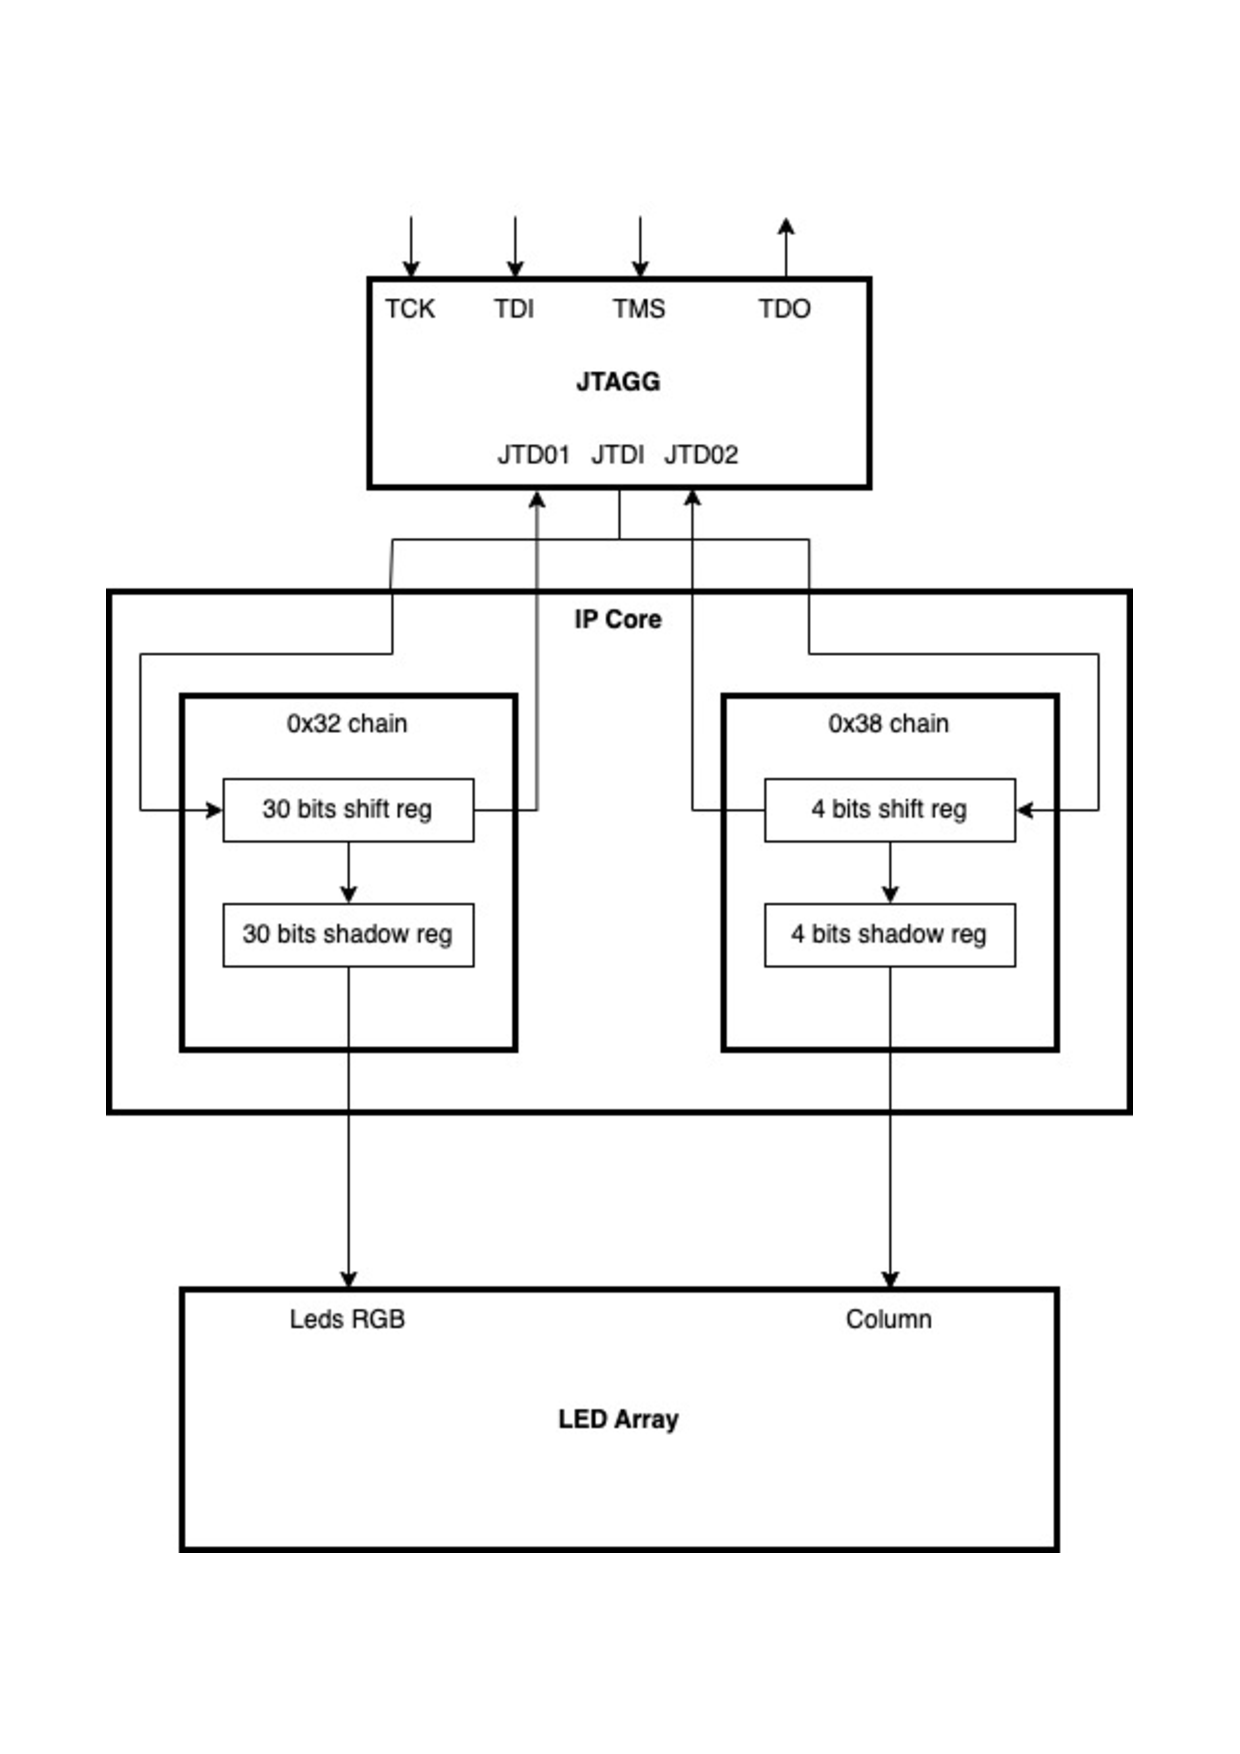
\includegraphics[width=0.85\linewidth]{figures/IPCORE_Design.pdf}
    \caption{Simplify block diagram of the \texttt{ipcore} and its integration}
    \label{fig:ipcore_block}
\end{figure}

A core concept behind these chain modules is the use of shift registers, which are fundamental to the serial communication via JTAG and use throughout this project.

Shift registers are digital circuits composed of a series of flip-flops that sequentially move data in or out, one bit at a time, synchronized with a clock.  
They enable efficient serial data transfer over minimal lines, which is ideal for FPGA environments with limited I/O.  
In our design, shift registers receive incoming data bit-by-bit from the host system, storing it temporarily for processing.  
To maintain reliable data handling, a shadow register captures the full data word once all bits are shifted in, enabling processing of complete instructions while continuing data reception.
  
Similarly, when sending data back to the host, values are loaded into the shift register and shifted out serially via the TDO line, synchronized to the JTAG clock.

Both \texttt{Chain1} and \texttt{Chain2} modules implement this mechanism: a shift register and a shadow register.  
Data shifting is enabled when \texttt{JSHIFT} is high and the corresponding instruction is active.  
Data is latched into the shadow register when \texttt{JUPDATE} is asserted.  
The shadow register output is then mapped to the relevant hardware outputs (RGB LED signals for \texttt{Chain1}, column selection for \texttt{Chain2}).

An important detail concerns the internal behavior of the \texttt{JTAGG} module regarding data input on the \texttt{TDI} pin.  
Unlike a direct pass-through, data bits pass through an internal flip-flop clocked by \texttt{JTCK}, introducing a one-cycle delay before the bits appear at the chain outputs.  
To compensate for this latency, shift registers can be seen as a register with an additional bit for the internal delay.  
For example, \texttt{Chain2}, which is logically implemeted using a 4-bit shift register, actually needs when communicating a shift of 5 bits to compensate JTAGG flip-flop.  
The first four bits correspond to the data, while the extra bit accounts for the internal \texttt{JTAGG} delay.  
This approach ensures proper alignment and availability of data despite the internal pipeline stage.

Overall, this design enables the ipcore to serve as a bridge between JTAG commands and low-level hardware control, providing a clean and modular interface to manipulate board components via the JTAG interface.

\subsection{How to communicate with the board through JTAG?} 
\label{sec:openocd}
Now that we have a clear understanding of the \texttt{JTAGG} module and the \texttt{ipcore}, we can describe how to communicate with the board via JTAG in practice.

First, the \texttt{.lpf} (lattice preference file) is updated to map the output signals of the two chains to the corresponding pins of the RGB LED matrix.  
Next, the updated design, containing both the \texttt{ipcore} and the \texttt{JTAGG} module, is synthesized and a bitstream is generated using the toolchain described in Section~\ref{sec:toolchain} by running the shell 
script at \texttt{JTAG\_support\_for\_Gecko5Education/project/scripts/synthesize.sh}.  
Once the bitstream is loaded onto the FPGA, OpenOCD can be used to interact with the board through JTAG.

After launching OpenOCD with a board-specific configuration file (\texttt{\$ openocd -f config.cfg}), it starts a local Telnet server on port \texttt{4444}.  
We can connect to this server and use the extensive command set it provides to interact with the board (\texttt{\$ telnet localhost 4444}).  
Although OpenOCD provides many commands, we focus here on a subset directly related to low-level JTAG operations, which are enough for the scope of this project:

\begin{itemize}
    \item \verb|irscan <tap_name> <instruction>|: This command shifts the instruction into the instruction register of the TAP controller and returns in RUN/TEST-IDLE state.
    \item \verb|drscan <tap_name> <size> <data>|: This command shifts the first \texttt{size} bits of the data into the data register corresponding to the loaded instruction and returns in RUN/TEST-IDLE state.
    \item \verb|pathmove <tap_state_name>|: This command moves the TAP controller to the specified state.
    \item \verb|runtest <nb_cycles>|: This command runs the TAP controller for \texttt{nb\_cycles} clock cycles.
\end{itemize}

To control the RGB LEDs, we begin by shifting either the \texttt{ER1} or \texttt{ER2} instruction into the instruction register using the \texttt{irscan} command.  
Then, the corresponding data, either the color values or the column selection, is sent using the \texttt{drscan} command.  
If necessary, the TAP controller can be reset using the \texttt{pathmove reset} command.

\subsection{Milestone 1 Conclusion}

This first milestone successfully demonstrates a minimal yet functional JTAG-based communication interface on the \boardName board.  
By leveraging the \texttt{JTAGG} module and a custom-designed \texttt{ipcore}, we were able to control the RGB LED matrix through two dedicated custom instructions.  
The modular design using shift and shadow registers provides a robust foundation for serial communication, while OpenOCD enables straightforward interaction with the board from a host machine.  
Overall, this milestone validates the feasibility of using JTAG as a flexible and extensible interface for on-board control, offering a solid proof of concept for the next milestone of the project.

\section{Milestone 2: Memory and Peripheral Access}

The second milestone uses the proof of concept established in the first milestone to extend the JTAG interface to support memory and peripheral access.

\subsection{The JTAG Interface Module}

This part of the project focuses on the design and integration of a Verilog module named \texttt{jtag\_interface}, which is added to the architecture introduced in Section~\ref{sec:arch}. 
This module serves as a bridge between the JTAG communication mechanism and the system's shared bus, allowing access to memory and peripherals.

To facilitate implementation, modularity, and reuse, the \texttt{jtag\_interface} is designed in a hierarchical and modular fashion. The global structure is as follows:

First, we instantiate the \texttt{JTAGG} module, which manages the JTAG protocol and implements the TAP controller.  
Directly connected to this block is the ipcore module, which provides and handles custom JTAG instructions as in the first milestone.  
These instructions allow the user to read from and write to the shared bus architecture.  

To perform actual bus transactions, the \texttt{ipcore} delegates control to a Direct Memory Access (DMA) module.  
This DMA module is directly connected to the shared bus of the architecture.  

For improved performance, data exchanged between the \texttt{ipcore} and the DMA module is buffered using a pingpong buffer.  
This buffer enables  parallel usage from the ipcore and the DMA and allows transactions to move chunks of data instead of single 32 bits words.

The high-level architecture of the JTAG interface module is illustrated in Figure~\ref{fig:big_picture}.

\begin{figure}
    \centering
    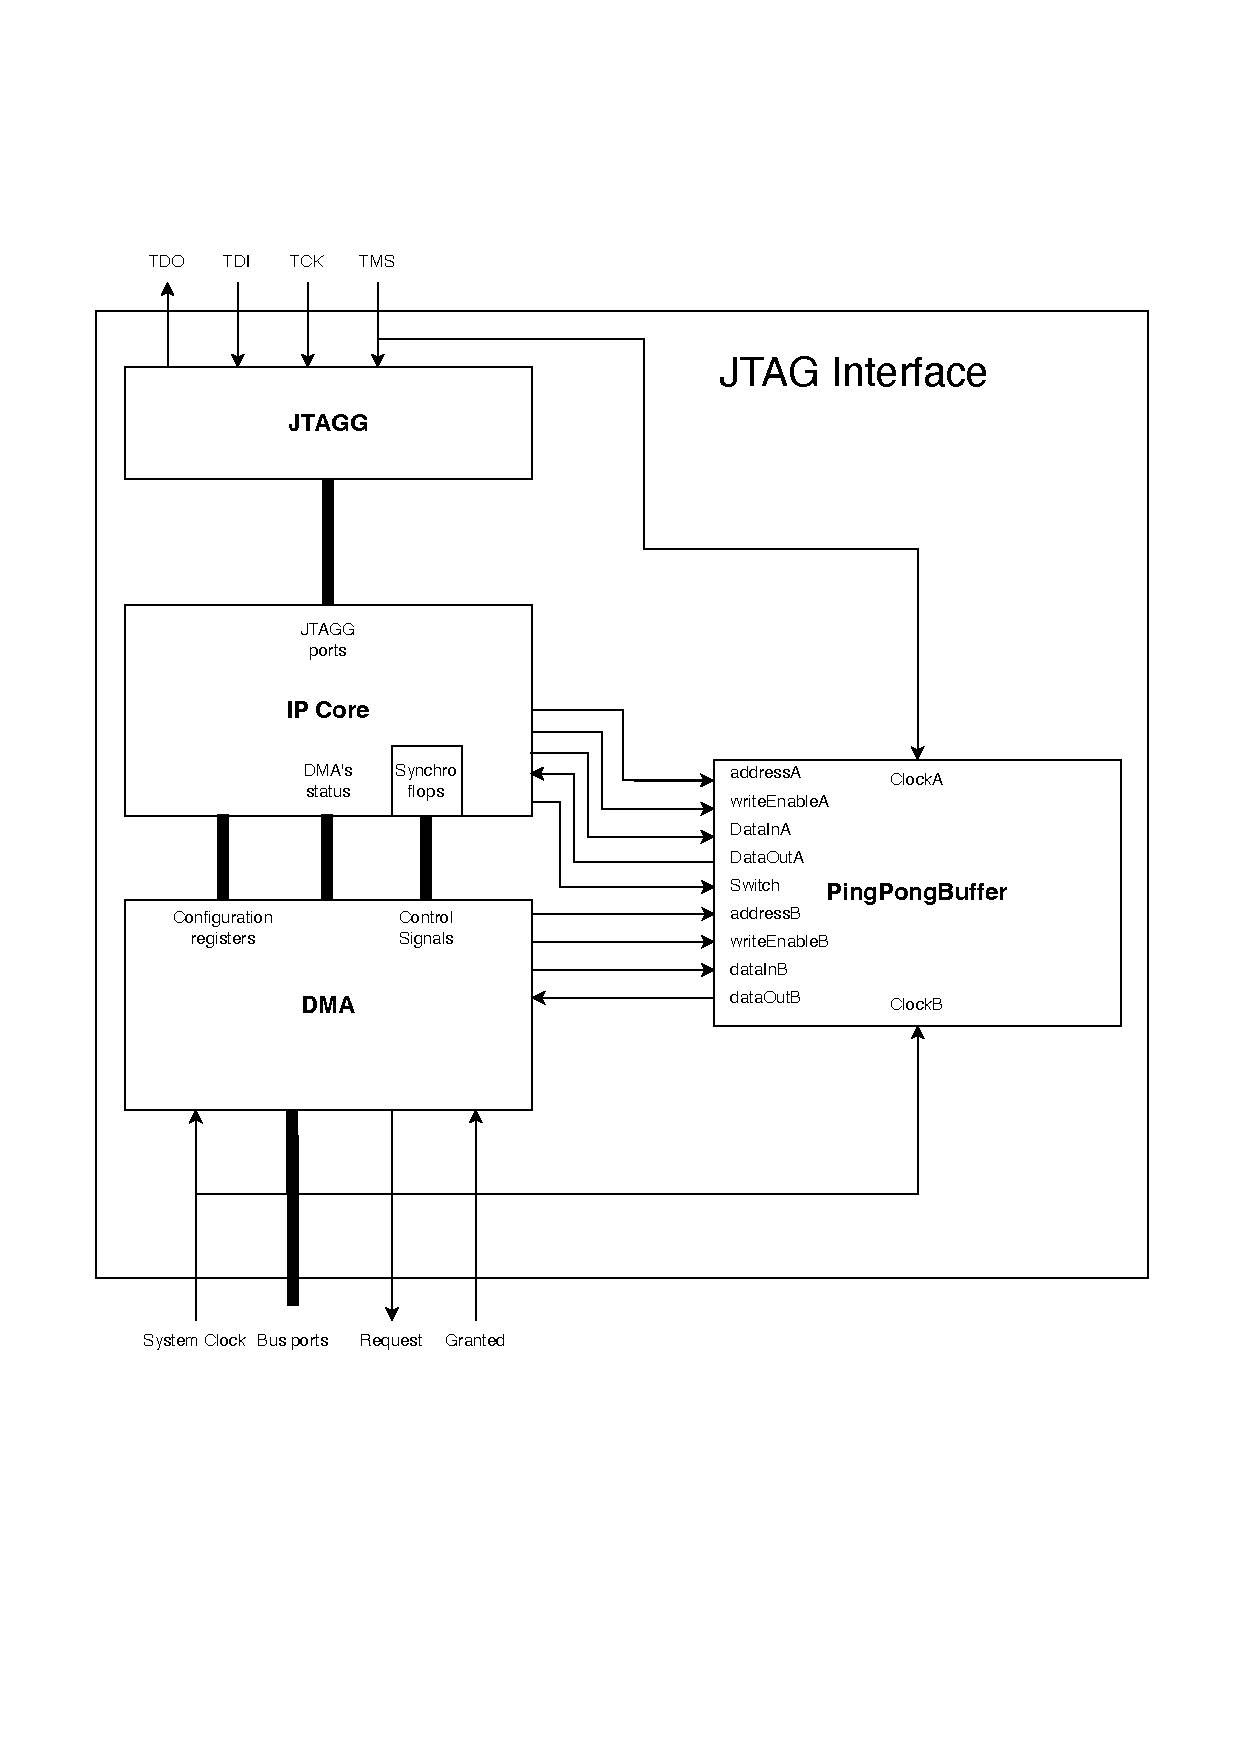
\includegraphics[width=0.9\linewidth]{figures/jtag_interface_overview.pdf}
    \caption{High-level architecture of the JTAG interface module}
    \label{fig:big_picture}
\end{figure}

Before diving into the internal design of the JTAG interface module, we will briefly describe the shared bus architecture it is supposed to communicate with.

\subsection{The Bus Architecture}

The shared bus architecture coordinates communication between multiple modules through a set of defined signals totaling 50 bits.
At its core, a 32-bit address\_data channel carries both addresses and data depending on the transaction phase.

The main control signals are:

\begin{itemize}
    \item \textbf{byte\_enables} (4 bits): Specifies which bytes in the transfer are valid.
    \item \textbf{burst\_size} (8 bits): Indicates the number of words transferred in a single burst.
    \item \textbf{read\_n\_write} (1 bit): Differentiates read and write operations.
    \item \textbf{begin\_transaction} and \textbf{end\_transaction} (1 bit): Mark transaction boundaries.
    \item \textbf{data\_valid}, \textbf{busy}, and \textbf{error} (1 bit): Status signals to manage data integrity and flow control.
\end{itemize}

The bus follows a master-slave model, where the master initiates and controls transactions, and the slave responds accordingly. It is
controlled by a bus arbitrer that manages access to the bus and ensures that only one master can communicate with the bus at a time.
This arbitrer has an input request signal for each master on the bus, and it outputs a grant signal to the selected master.

All signals are active-high and must be cleared (set to zero) when idle to avoid glitches caused by the bus’s logic design. 
This design supports flexible and efficient data exchange among connected modules.

We will now enter into more details about the design of each of the submodules of our JTAG interface module.

\subsection{The ipcore}

The first milestone demonstrated that the JTAG interface can be used to enable meaningful communication with the board, thanks to a simple ipcore that translates JTAGG signals into concrete actions on the board.

In this second milestone, the ipcore retains the same core role, but is completely redesigned to support reading and writing data over the shared bus architecture.

In this new design, the ipcore includes multiple interfaces to communicate with other components of the JTAG interface module.  
First it interfaces with the JTAGG module to receive data from the host system and send data back.
It also has an interface to communicate with the DMA module, which allows the ipcore to initiate the DMA's operations, send the bus operation configurations and 
receive status feedback from the DMA module.
Finally, the ipcore interfaces with the pingpong buffer allowing it to read and write data from the buffer's parts and to switch them, facilitating the data exchange between the DMA and the ipcore.

In this milestone, the ipcore uses only one of the two custom instructions provided by JTAGG (the \texttt{0x32} instruction).  
Therefore, only the Chain1 module is instantiated within the ipcore, leaving Chain2 unused and available for future functionality.

Once the instruction ER1 is loaded into JTAGG instruction register, the user can communicate with the ipcore using serial data in and out signals by sending 
 ipcore defined commands.
Those commands are part of a set of commands enabling operations such as writing or reading configuration registers, transderring data to/from ipcore's part of the pingpong buffer,
and launching the DMA read or write operation on the bus.

To simplify the design and usage, all instructions use a fixed length composed of two parts:
The first part is the data section, which some instruction uses to provide data to the ipcore.
The second part is the command operand, specifying the command to be executed.

Choosing 32 bits for the data section matches the bus and buffer word size, enabling whole words or addresses to be transferred in a single instruction.  
The 4-bit opcode allows for up to 16 commands, which suffices for this design.
The total instruction length of ipcore's commands is 36 bits.

The commands are the following:

\begin{table}[h!]
    \centering
    \begin{tabular}{|c|c|p{8cm}|}
        \hline
        \textbf{Data Section (32 bits)} & \textbf{Opcode (4 bits)} & \textbf{Usage} \\
        \hline
        -                               & 0000                     & No operation (used to shift out data) \\
        Address $[35:4]$                & 0001                     & Write start bus address \\
        Byte Enable $[7:4]$             & 0010                     & Write bus byte enable \\
        Burst Size $[11:4]$             & 0011                     & Write bus burst size \\
        -                               & 0100                     & Read start bus address \\
        -                               & 0101                     & Read bus byte enable \\
        -                               & 0110                     & Read bus burst size \\
        -                               & 0111                     & Reserved \\
        Word $[35:4]$                   & 1000                     & Write word into ping-pong buffer and increment block size \\
        -                               & 1001                     & Read next word from ping-pong buffer \\
        -                               & 1010                     & Launch DMA write operation (when ready) \\
        Number\_of\_words $[11:4]$      & 1011                     & Launch DMA read operation for specified number of words (when ready) \\
        -                               & 1100                     & Wait for DMA completion and switch buffer \\
        -                               & 1101                     & Reserved \\
        -                               & 1110                     & Reset the Buffer signals (including the block size) \\
        -                               & 1111                     & Reset the ipcore \\
        \hline
    \end{tabular}
    \caption{JTAG ipcore Command Set: Data section, opcode, and usage.}

\end{table}

The ipcore design is structured around several key registers. 
The Bus Start Address Register specifies the starting address for bus operations, 
while the Bus Byte Enable Register determines which bytes within a word are active during transfers 
(with all bytes enabled by default). 
The Burst Size Register sets the number of words to be transferred before the bus is released, 
and the Block Size Register keeps track of the number of valid words in the ipcore's section of the pingpong buffer, 
as well as the number of words involved in DMA bus operations.

The Shift Register manages serial instruction shifting, similar to Milestone 1, but now when \texttt{JCE1} is high, it can load data from the status register, configuration registers, or pingpong buffer based on the previous command.
This enables the user to request and retrieve data from the ipcore.

The Status Register reports the current \texttt{ipcore} state, including flags indicating whether the byte enable, burst size, and bus address registers are loaded; the current block size; DMA busy status; and whether the DMA operation has completed.

\begin{figure}
    \centering
    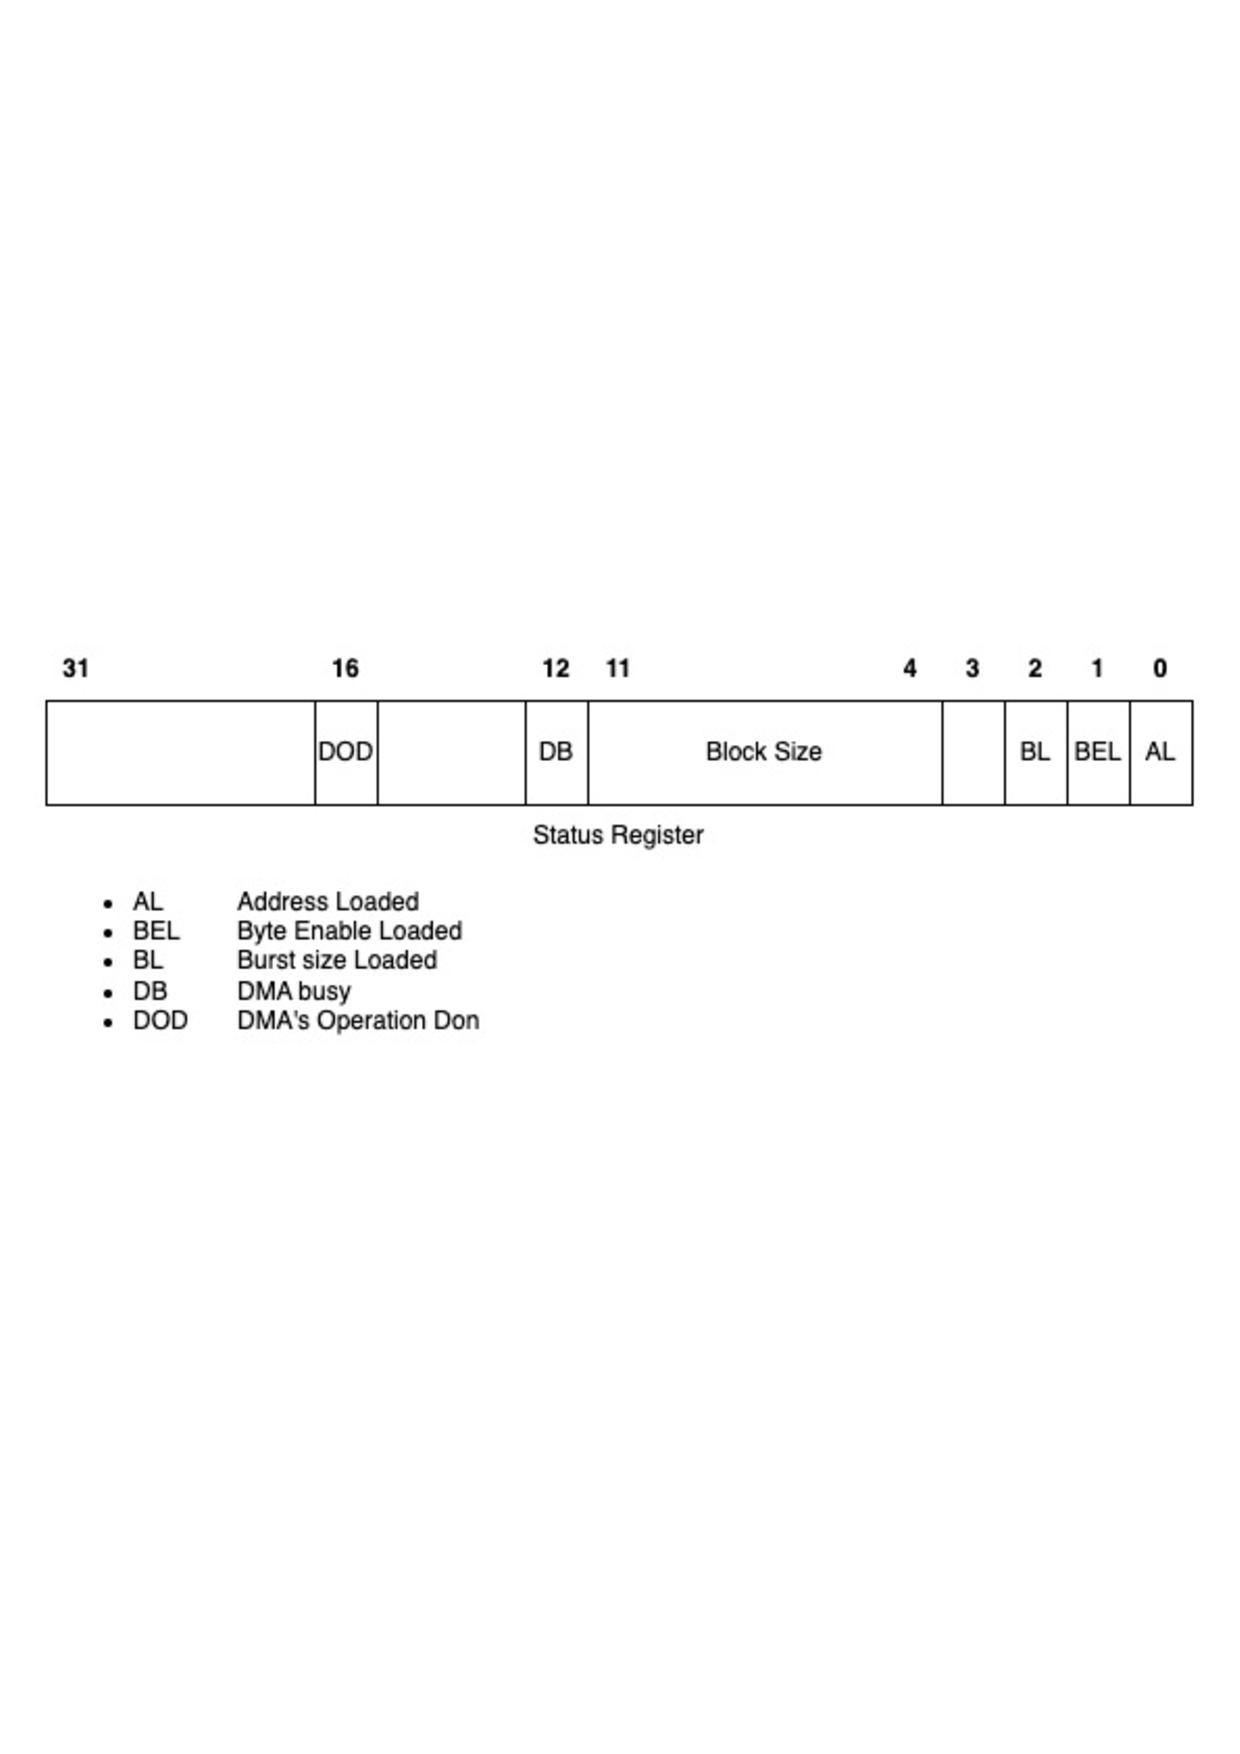
\includegraphics[width=0.9\linewidth]{figures/status_reg.pdf}
    \caption{Status register of the \texttt{ipcore}}
    \label{fig:status_register}
\end{figure}

Internally, the \texttt{ipcore} uses a finite state machine (FSM) to manage command execution timing and behavior. It is provided on Figure~\ref{fig:ipcore_fsm}.

\begin{figure}
    \centering
    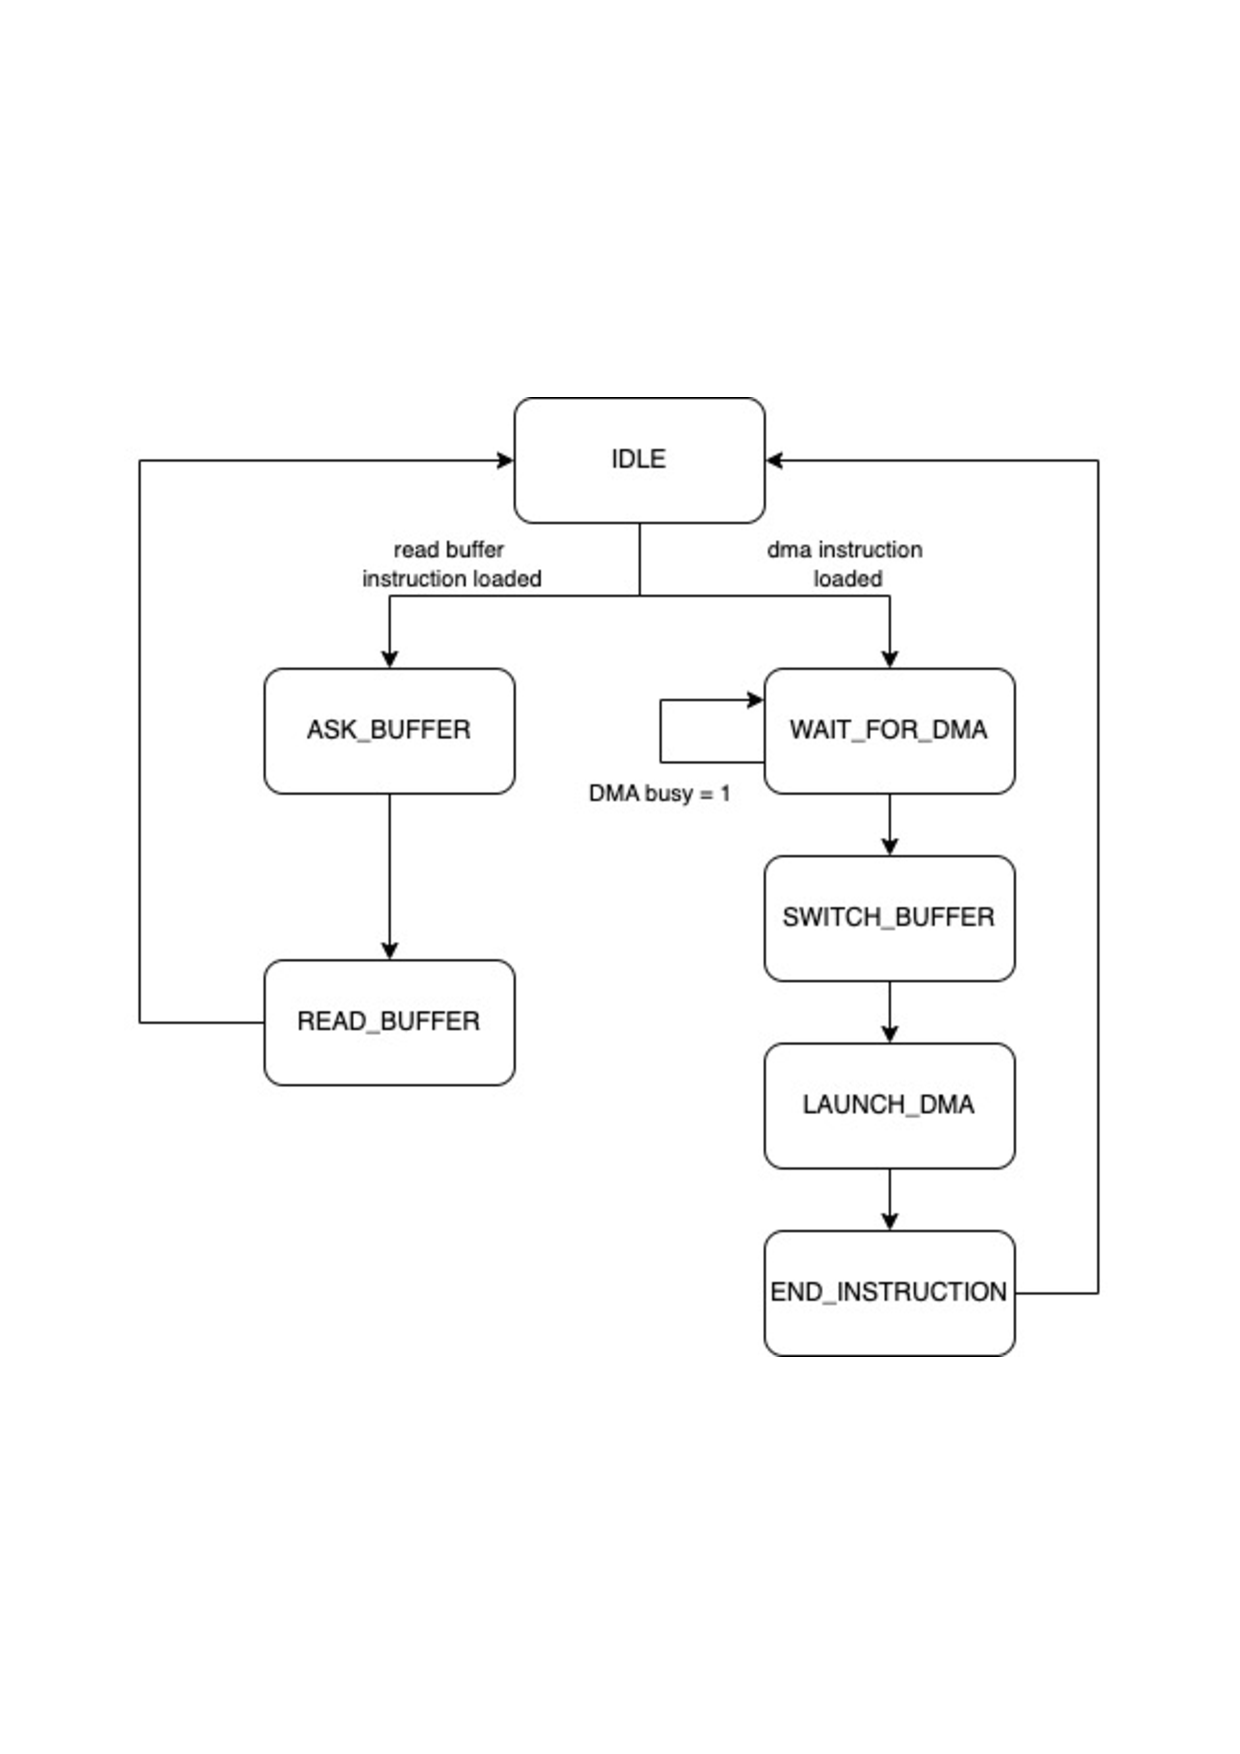
\includegraphics[width=0.9\linewidth]{figures/ipcore_fsm.pdf}
    \caption{Finite state machine of the \texttt{ipcore}}
    \label{fig:ipcore_fsm}
\end{figure}

The first state is the \texttt{IDLE} state, where the \texttt{ipcore} waits for a new command to be issued.
Most of the time, the FSM remains in this idle state. In fact, writing to any configuration register is done
in the same clock cycle as the command is latched into the shadow register (when \texttt{JUPDATE} is high),
so there is no need to leave the idle state for such operations.

Similarly, the write-to-buffer operation does not require a state change.
Although the write is not performed in the exact same cycle as the command is received,
it is handled in the following cycle by internal logic. This logic updates the block size register,
prepares the data, and selects the correct buffer address for the write using internal signals and registers.
Even though there is a slight clock delay between receiving the command and completing the write,
this has no negative impact on the design. Shifting the next instruction takes 37 clock cycles
(32 bits for data, 4 bits for the opcode, and one additional shift as explained earlier),
leaving sufficient time for the write operation to complete before next command is latched.

The read-from-buffer operation, however, is more complex and does require a state change.
Intuitively, reading from the buffer involves two steps:
first, setting the buffer address, and then retrieving the data from that address.
After that, the data must be moved to the shift register for output to the host system.
This is implemented by transitioning to the \texttt{ASK\_BUFFER} state, where the read address is set up.
The FSM then proceeds to the \texttt{READ\_BUFFER} state, which handles the actual data read
and places the result into the shadow register.
In the next clock cycle, the data can be captured by the shift register, and the FSM returns to the \texttt{IDLE} state.
To retrieve the data, the user must shift it out by issuing any new instruction.
\textbf{Important note: It is the user's responsibility to wait three clock cycles for the result of the read from buffer operation
to be ready to be captured and later shifted out of the shift register.} This delay can be handled in OpenOCD using the \texttt{runtest 3} command.

The final part of the finite state machine handles DMA-related operations,
all three of them follow a similar state sequence.
First, the FSM enters the \texttt{WAIT\_FOR\_DMA} state, where it waits until the DMA is no longer busy.
Once the DMA is ready, the FSM transitions to the \texttt{SWITCH\_BUFFER} state.
Here, the ping-pong buffer parts are swapped: the half previously used by the DMA
becomes accessible to the ipcore, and inversely.
This allows the ipcore to access the results of a DMA read operation,
or prepare data for the DMA to write to the bus.
After switching buffers, the FSM moves to the \texttt{LAUNCH\_DMA} state,
where it initiates the appropriate DMA operation by asserting one of three output signals:
launch\_read, launch\_write, or only\_switch.
The read operation starts the DMA read process, the write operation
initiates the DMA write process and the only switch operation simply switches the buffers without launching a DMA operation.
Before returning to the \texttt{IDLE} state, the FSM enters the \texttt{END\_TRANSACTION} state
to reset internal control signals and prepare for the next instruction.

\textbf{Important note: As with reading buffer data, the user must ensure the DMA is ready before issuing a DMA command.}
Since the clock driving the FSM is user-defined, the user must periodically check the status register
until the DMA is no longer busy.

This concludes the high level design of the finite state machine used in our new ipcore.

However, there are still more important lower level aspects to mention. 
First, at the time data is captured in the shift register before being shifted out, 
the ipcore has no knowledge of the instruction being shifted in. 
This implies that to retrieve data from the ipcore, such as configuration registers 
or the contents of the ping-pong buffer, the user must first shift in the instruction that initiates the read. 
Then, they must shift for 37 clock cycle again to retrieve the data, this can be done by sending any instruction.
For this purpose, the \texttt{0x00} instruction can be used. 
It acts as a no-op and simply captures and shifts out the current data without triggering any action in the ipcore.

For the same reason, the status register is only received updated when the next instruction is shifted in. 
We can consider the status register to reflect the state of the ipcore 
at the moment the previous instruction completed execution. 
For example, after a DMA-related instruction, 
the ipcore's block size register may already be updated by the DMA, 
but the status register will still display the old value until the following instruction is shifted in.


Second, as previously explained, the block size register serves a dual purpose:
it indicates both the number of words currently stored in the \texttt{ipcore}'s half of the ping-pong buffer,
and the number of words involved in a DMA bus transaction.
This dual use implies a limitation. If the user attempts to read or write more than the buffer's capacity (1KB), 
the ipcore will ignore the excess data. When this happens, instead of transferring further words,
it will begin shifting out the status register.

Third, some instructions come with specific preconditions. 
In particular, the DMA launch instructions, both read and write, require the block size register to be non-zero.
For a write operation, this means that the user must have written data to the buffer before launching the DMA.
For a read operation, the user must indicate how many words should be read by using the data section of the command.

This nearly completes our description of the new ipcore's logic and architecture. 
As demonstrated, it is a simple yet powerful module, giving the user full control over both the pingpong buffer and the DMA module, providing efficient data transfer to and from the bus.
Moreover, the design is modular and extensible. 
It can be adapted for other use cases simply by modifying the command set and the associated logic.

To properly finalize this module, there remains one critical issue to address:
the presence of two independent clock domains. 
The next subsection will explain how this challenge is resolved in our design.

\subsection{The Two Clock Domains Problem}

In this milestone, a new challenge emerges that was not present in the earlier stage of development: the two clock domains problem. 
Now that our design interfaces with an actual microcontroller architecture running on the board, 
we need to paid attention to the distinct clock domains involved.

On one side, the JTAG clock (\texttt{TCK}) is used to synchronize both the JTAGG block and the ipcore. 
On the other side, the system bus architecture is clocked by a different signal—\texttt{system\_clock}—which is also used by the microcontroller. 
Consequently, the DMA which communicates with the bus must also be clocked by \texttt{system\_clock}. 
Since these clocks are not synchronized, especially the JTAG clock, which is entirely under user control, it becomes critical to handle timing with care.

Because the ipcore and the DMA reside in different clock domains, communication between them must be carefully analyzed. 
Fortunately, not all communications require synchronization. For instance, configuration registers can be safely read by the DMA at any time, 
as they remain constant during the DMA launch. The DMA can simply capture their values once and store them internally for later use.
Similarly, data transfer via the pingpong buffer does not require clock domain synchronization. 
This is thanks to the buffer's design, which is inherently capable of handling two clock domains.

The only signals that require proper synchronization are the DMA control signals, the ones that trigger DMA operations. 
To safely transfer these signals across clock domains, the ipcore employs what are known as \texttt{synchronous flops}. 
These are implemented using a three-stage synchronizer, which ensures that a signal high for one clock cycle in the input domain 
appears high and stable for exactly one clock cycle in the output domain, avoiding metastability and undefined behavior.

The synchronizer's operation is straightforward. The signal is first passed through a flip-flop clocked by the input domain. 
To ensure it remains high until explicitly cleared, the input of this flip-flop is ored with its own output. 
This holds the signal high until reset.
Next, the signal passes through two additional flip-flops, both clocked by the output domain. 
These serve to synchronize and stabilize the signal in the new clock domain. 
Once the output is high, the first two flip-flops are asynchronously reset, 
guaranteeing that the signal stays high for a single cycle of the output domain.
The detailed schematic of the synchronizer is presented in Figure~\ref{fig:sync}.

\begin{figure}
    \centering
    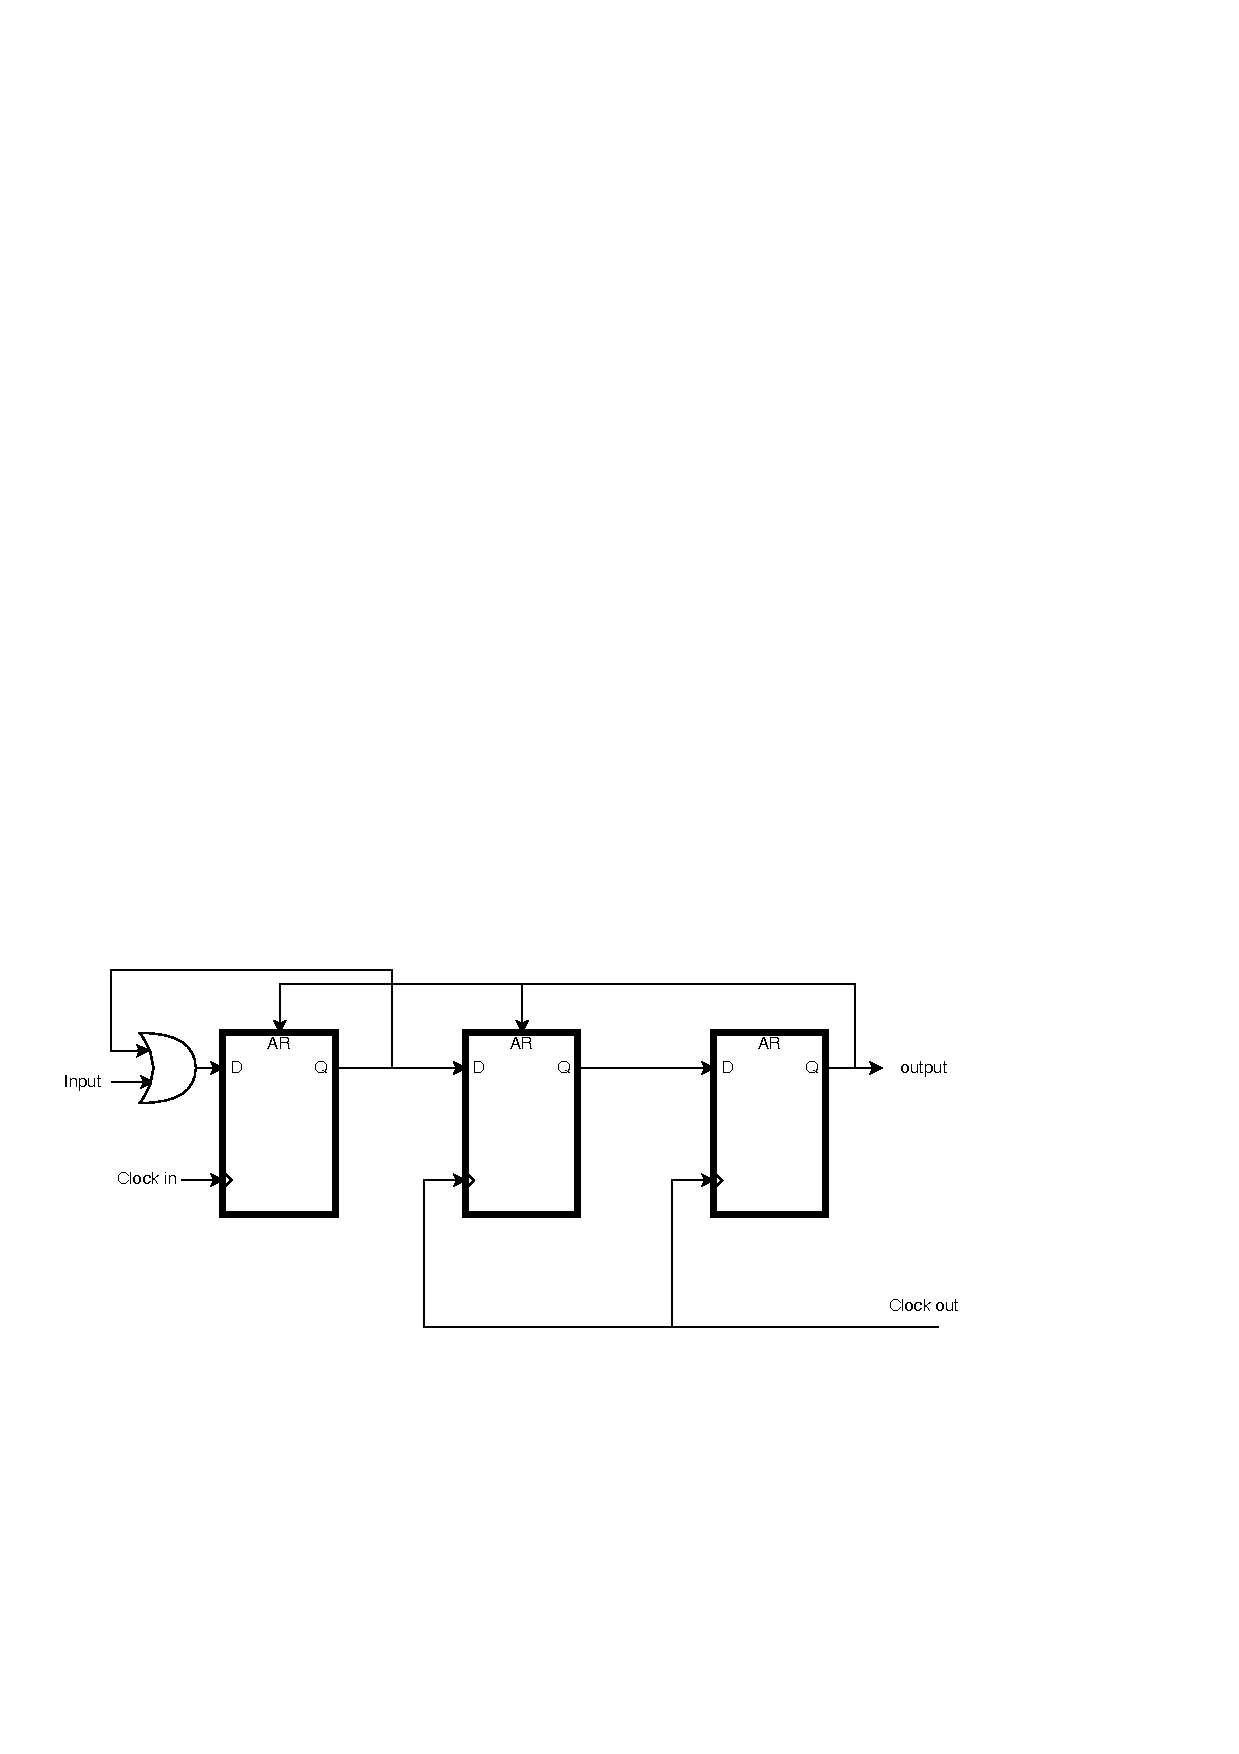
\includegraphics[angle=-90, width=\linewidth]{figures/clock_synchronizer.pdf}
    \caption{Schematic of the synchronizer used in the ipcore to safely transfer control signals across clock domains.}
    \label{fig:sync}
\end{figure}

This synchronization scheme is applied three times in the ipcore design: 
once for the DMA read launch signal, once for the DMA write launch signal, and once for the pingpong buffer switch command.

With this, the \texttt{ipcore}'s design is complete. It is now fully capable of safely communicating with both the buffer and the DMA module. 



\subsection{The pingpong buffer}

The pingpong buffer is not a complex design, but it is a key component of this second milestone. 
It serves as an intermediate storage area between the ipcore and the DMA module, 
with the particularity that both components can access it concurrently. 
For instance, the DMA could be reading data from the buffer to write to the bus, 
while at the same time the ipcore is writing new data to prepare for the next DMA transaction. 
The core idea is to have two memory regions, one allocated to each component, and to be able to switch them at any moment. 

This is achieved using a fully dual-ported SSRAM, which supports simultaneous access from two independent interfaces. 
Each interface includes its own set of signals: address lines, input data, output data, a read/write control (high for read, low for write), and a dedicated clock. 
These two interfaces are completely independent, allowing the ipcore (clocked by \texttt{TCK}) 
and the DMA (clocked by \texttt{system\_clock}) to operate concurrently and safely, 
thereby addressing part of the clock domain crossing problem described in the previous section.

It is also important to note that due to the synchronous nature of the memory, 
any data written to or read from the pingpong buffer becomes valid after one clock cycle. 
This means that a write operation will take one clock cycle before the data is stored and accessible, 
and similarly, data read from the buffer will be available one clock cycle after the address is issued. 

The pingpong buffer ensures that this dual-ported memory is logically divided into two regions. 
This is done by forcing the most significant address bit to 0 or 1, depending on the interface. 
In doing so, the ipcore is restricted to one half of the memory, 
and the DMA to the other which guarante mutual exclusion. 
Switching buffers simply involves inverting this most significant bit, effectively swapping buffer halves between the two components.

The used version in this milestone also includes an input signal, handled by the ipcore, 
which triggers the buffer switch on the rising edge of the JTAG clock. 
This allows the buffer regions to be exchanged when the ipcore requests it.

In our design, the pingpong buffer uses a 2KB dual-ported memory, word-addressable in 32-bit words. 
This means each half of the memory provides 1KB (128 words) to the ipcore and DMA respectively. 
As a result, the buffer can handle a total of 256 words, and addresses are 8 bits wide, the 9th bit being reserved for partitioning.

This size was chosen for practical reasons. 
First, it meets the data throughput needs of this project. 
Second, increasing it further would not significantly improve performance, since buffer switching is fast and efficient. 
Finally, 2KB is the largest usable configuration on our FPGA without moving to inefficient implementations based on flip-flops and multiplexers.

In conclusion, the pingpong buffer enables efficient and concurrent data exchange between the ipcore and the DMA. 
It respects clock domain boundaries while remaining lightweight, robust, and easy to integrate into the rest of the system.

\subsection{The DMA Controller}

The Direct Memory Access controller (DMA) is probably the main component of this new design.  
It is responsible for executing the bus operations requested by the ipcore.  
The DMA module is a Verilog component whose ports can be divided into four groups.  
First, there are the ports used to communicate with the ipcore, including control signals, configuration registers, and some status signals.  
Then, there are twelve ports used to act as a master on the bus architecture and communicate with the bus.  
Additionally, two ports connect to the bus arbiter; these are used to request the bus and acknowledge bus access.  
Finally, some ports communicate with the pingpong buffer to allow read and write operations to be performed on it.

Conceptually, the DMA module should handle both read and write operations on the bus.  
Data read from the bus should be written to the pingpong buffer,  
and data written to the bus should be read from the pingpong buffer (previously written by the ipcore).  
The best way to achieve this is by using a finite state machine (FSM) that handles the timing of operations and bus access.

The finite state machine of the DMA is complexe and we will walk through it state by state.
For the ease of the explanation, a state diagram is shown in Figure~\ref{fig:state_diagram}.

\begin{figure}
    \centering
    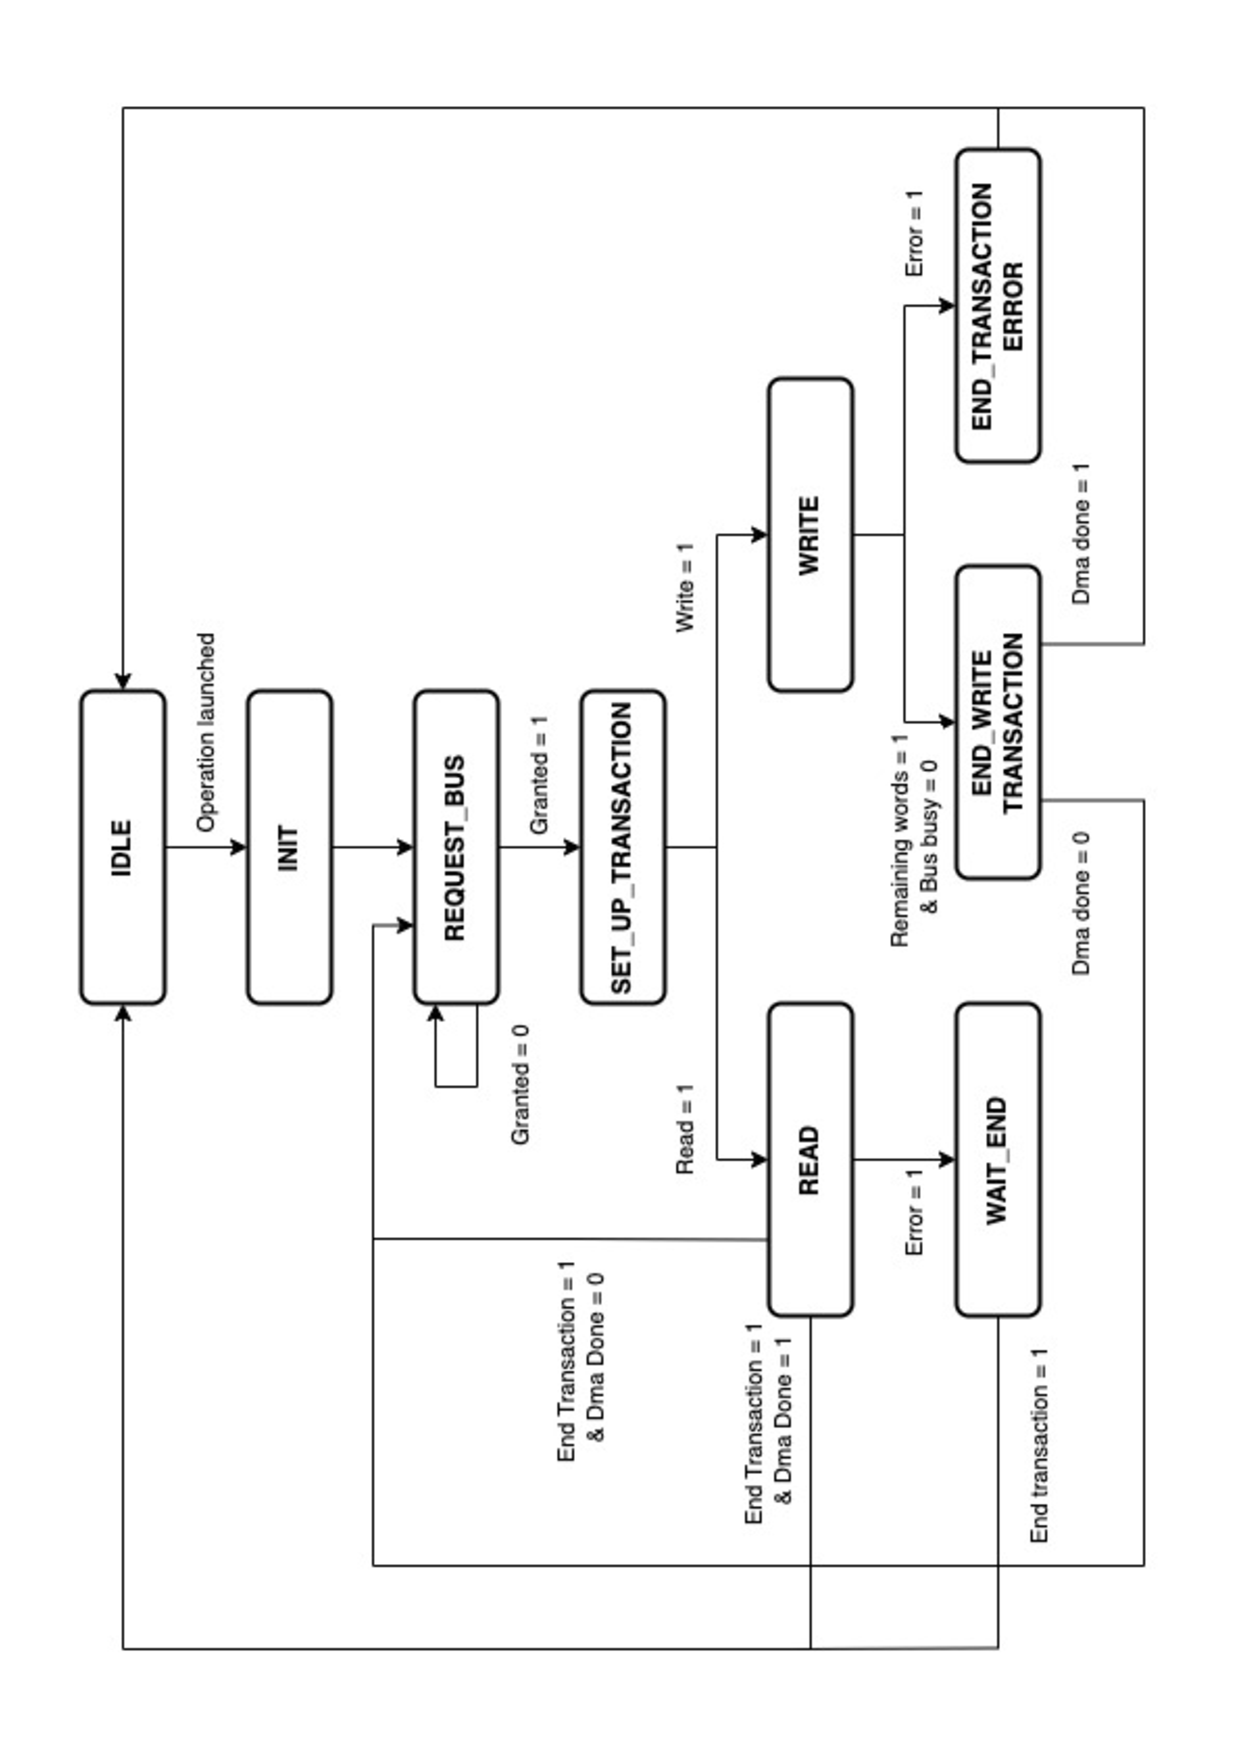
\includegraphics[angle=-90, width=0.9\linewidth]{figures/dma_fsm.pdf}
    \caption{Finite state machine of the DMA controller}
    \label{fig:state_diagram}
\end{figure}

The first state entered when the DMA is reset is the \texttt{fsm\_idle} state.  
In this state, the DMA is idle and waits for control signals from the ipcore to start a new operation.  
It is the only state where the DMA is not busy, and a new operation can be launched.  
Once a start signal is received, the DMA reads the ipcore's configuration registers, stores a copy,  
records the type of instruction in a register, and transitions to the \texttt{fsm\_init} state.  
The saved configuration registers include the start address for the bus operation, burst size, byte enable signals, and the number of words to be read or written.

The \texttt{fsm\_init} state initializes all the registers needed for a single DMA operation.  
Three registers are especially important:  
\texttt{updated\_bus\_start\_address\_reg} holds the next bus address for the operation and is initialized to the stored start address.  
\texttt{Updated\_block\_size\_reg} holds the remaining number of words to read or write and is initialized to the stored block size.  
\texttt{Pp\_address\_reg} stores the next pingpong buffer address for data transfer and is initialized to \texttt{0x0}.  
Two more registers are updated to inform the ipcore whether the operation has started and whether it has finished.  
After one clock cycle in this state, all registers are initialized, and the DMA moves to the \texttt{fsm\_request\_bus} state.

In the \texttt{fsm\_request\_bus} state, the DMA asserts its bus request signal to start an operation.  
It waits in this state until the bus arbiter grants bus access, once granted the DMA proceeds to the \texttt{fsm\_set\_up\_transaction} state.

According to the shared bus architecture used in this project, the first clock cycle of any bus operation is used to set up the transaction.  
The \texttt{fsm\_request\_bus} state configures the bus control signals, including byte enable, burst size, and read/write indication, based on the configuration registers and operation type.  
The DMA also sets the begin transaction signal high to indicate the start of the transaction,  
and sets the \texttt{address\_data} signal to the value of the updated bus start address register.  
If the operation is a read, an internal register is also initialize to store the actual number of words to transfer in the burst.  
This value is set to the burst size received from the ipcore if it is smaller than the remaining block size; otherwise, it is set to the remaining block size.  
Once this setup is complete, the DMA transitions to either the \texttt{fsm\_read} state (for reads) or the \texttt{fsm\_write} state (for writes).

The \texttt{fsm\_read} state handles reading data from the bus and writing it to the pingpong buffer.  
When valid data is detected on the bus, the DMA updates the \texttt{updated\_bus\_start\_address\_reg} by adding 4 (the size of a word),  
decrements the \texttt{updated\_block\_size\_reg} by one,  
and increments the \texttt{pp\_address\_reg} to the next pingpong buffer address.  
It stores the read data in a temporary register connected to the pingpong buffer data input,  
and sets the write enable register high so the data will be written to the buffer on the next clock cycle.  
The DMA remains in this state until it receives an end transaction signal from the slave or an error signal from the bus.  
In case of an error, the DMA transitions to the \texttt{fsm\_wait\_end} state, where it stalls until the end transaction signal is received, then returns to \texttt{fsm\_idle}.  
If the transaction ends normally, two scenarios are possible:  
either all data has been received, so the DMA returns to \texttt{fsm\_idle},  
or not all data was received (e.g., due to burst size limitations), in which case the DMA requests the bus again by moving back to \texttt{fsm\_request\_bus} and reapeat the same process until all data is received.

The \texttt{fsm\_write} state is responsible for writing data from the pingpong buffer to the bus.  
In this state, the DMA stalls if the slave is busy (indicated by the \texttt{busyIn} signal).  
Otherwise, it updates the \texttt{updated\_bus\_start\_address\_reg}, \texttt{updated\_block\_size\_reg}, and \texttt{pp\_address\_reg} in the same way as in the read state.  
It also decrements the counter tracking the number of words left to write in the current burst.  
The DMA ensures that on every clock cycle, the data read from the pingpong buffer is driven to the bus data out port, and the data valid signal is asserted.  
Although reading from the buffer has a one-cycle delay, this is not an issue because the buffer reads by default data from the address in \texttt{pp\_address\_reg}.  
As a result, the first data written to the bus corresponds to the data at the current \texttt{pp\_address\_reg} address and has beed read since the \texttt{fsm\_init} state, after which the address register is incremented. 
This ensures that on each subsequent clock cycle, the next data word is available for sending on the bus.

There are two ways to exit this state.  
First if an error signal is received from the bus, the DMA moves to the \texttt{fsm\_end\_transaction\_error} state, sends the end transaction signal to the bus, and returns to \texttt{fsm\_idle}.  
If the number of words left to write in the burst reaches one and the bus is not busy, the DMA moves to the \texttt{fsm\_end\_write\_transaction} state.  
Depending on whether there are more words left to write for this transaction, the DMA either returns to \texttt{fsm\_idle} or to \texttt{fsm\_request\_bus} to requests the bus again and send another burst.

This concludes the detailed explanation of the DMA FSM.  
Since the rest of the design is simple combinational and sequential logic, we will not detail it here.  
To summarize, the DMA module waits for the ipcore to launch a new operation, initializes registers for the operation, and requests the bus.  
Once the bus is granted, it sets up the transaction and proceeds to either the read or write state.  
In the read state, data is read from the bus and written to the pingpong buffer;  
in the write state, data is read from the pingpong buffer and written to the bus.  
These bursts continue until the entire data block is transferred.  
Upon completion, the DMA returns to idle, clears the busy signal, set high the operation finished signal, and waits for the next operation.

This module greatly improves our design by allowing the ipcore to perform bus operations while preparing the next operation or processing previous results.  
It also enhances the understandability of the ipcore by encapsulating all bus timing and protocol complexities within a simple module.

This concludes the complete design of the JTAG interface module,  
where the JTAG block, the ipcore, the pingpong buffer, and the DMA controller are connected.  
Once it is integrated with the actual architecture, the user will be able to read and write data from memory or any peripheral connected to the bus.

\subsection{Integration to the architecture}

The integration of the JTAG interface module into the architecture is done by simply connecting the module to the bus architecture.  
In the existing setup, the bus arbiter provides a 32-bit wide signal for master requests (\texttt{s\_busRequests}) and a 32-bit wide signal for master grants (\texttt{s\_busGrants}).  
Since the architecture already includes four masters, the JTAG interface module is added as a fifth master by connecting the 27th bit of \texttt{s\_busRequests} and \texttt{s\_busGrants}  
to the request and grant signals used by the DMA module.  

To complete the integration into the bus architecture, all other signals coming from the DMA to the bus are ORed with the corresponding signals from the other masters.  
Which is the way our shared bus architecure is designed to handle multiple masters.
Finally, the signals coming from the bus are simply connected to the DMA module, and the system clock is drived to all component of the JTAG interface module.

This integration is straightforward and does not require any additional logic, as the JTAG interface module is designed to fit seamlessly into the existing bus architecture.
With this integration, the JTAG interface module can now communicate with the bus and perform read and write operations on the architecture.

\subsection{Implementation issue}

The current design of the JTAG interface module for the second milestone is actually a refactored version of an initial implementation that did not function correctly.  
In this subsection, we explain the issues we encountered in the first version and how the revised design addresses them.

The initial design followed the same general structure, comprising the JTAGG block, the ipcore, the pingpong buffer, and the DMA controller.  
However, the main differences lie in the design decisions made for the ipcore.

One of the biggest problems was the structure of the code itself. It was poorly organized and difficult to follow, making the system very hard to debug.  
This applied to both the ipcore and the DMA controller.  
Therefore, the first step in the redesign process was a full code refactoring to improve readability and maintainability.

The second major issue was the design of the ipcore.  
It was not well thought out, which made the system more complex, less intuitive, and provided very little feedback to the user.  
Even when functional, the previous design only allowed the user to read or write a single word at a time.  
It was also impossible for the DMA to perform bus operations simultaneously while the ipcore accessed the pingpong buffer.

An other clear example of the design limitations was the instruction set of the ipcore.  
It included only few operations: configuration register setup, a combined "write" command that handled both writing to the buffer and launching a DMA write,  
a "read" command for retrieving DMA results, and a command to start a DMA read.  
From a performance standpoint, this approach could have been efficient, as it required fewer instructions for data transfers.  
However, the internal logic was overly complex and difficult to debug.  
After considerable time trying to make the design work on hardware and following a meeting with my supervisor, I decided to rework the design entirely.

The main goal of the redesign was to simplify both the logic and the code.  
Previously, the FSM in the ipcore had separate paths for read and write operations.  
In the new design, all DMA transactions follow a unified path through the FSM, greatly simplifying the flow and making it easier to understand.

Additionally, the new design deliberately trades some performance for better usability, clarity, and debuggability.  
To achieve this, the ipcore now offers a broader and more specific command set.  
Instead of one command handling both buffer writing and DMA activation, commands have been split into smaller operations.  
For instance, there are now separate commands for controlling the pingpong buffer and for controlling the DMA.  
This provides finer control and makes the workflow more transparent.

The user is now responsible for writing data to the buffer before launching a write operation,  
or switching the buffer and reading from it after completing a read operation.  
While this slightly complicates usage, it is expected that a software layer interfacing with the JTAG interface will handle this logic rather than the user directly, as the evalution program does in 
Section~\ref{sec:evalution_program}.

This new breakdown of responsibilities also allows the ipcore to remain active while the DMA performs bus operations,  
enables multi-word transfers, supports burst configurations, and provides more visibility into the internal state of the system.

Finally, the new design introduces several improvements for debugging, one of the lacking areas in the previous version.  
These include the ability to read back values from the configuration registers,  
clearly distinguish between pingpong buffer operations and DMA transactions, reseting the buffer and the ipcore independently, 
and access a more informative status register that reflects both the DMA and buffer states.

In summary, while the new design may sacrifice a degree of raw performance compared to a fully optimized first version,  
it is significantly more robust, easier to debug, more user-friendly, and better suited for future extensions.

\subsection{Using the JTAG interface module}

The JTAG interface module is used in the same way as in the first milestone, through OpenOCD and its JTAG-related commands.  
However, since this milestone introduces more complexity, we provide a detailed example of how to read from and write to the bus using the JTAG interface module.

Once the design is loaded onto the board and the Telnet server is started, as explained in Section~\ref{sec:openocd}, the user can connect to the server using Telnet.

\vspace{1em}
\noindent\textbf{Example: Reading three words from address \texttt{0x00010000} using a burst size of 2}
\begin{lstlisting}
> telnet localhost 4444
> irscan ecp5.tap 0x32              // Select chain 1

// Set up the configuration registers
> drscan ecp5.tap 37 0x000100001    // Set bus start address
000000000
> drscan ecp5.tap 37 0xF2           // Set byte enable (optional, default is 0xF)
000000001                           // Status register: address loaded
> drscan ecp5.tap 37 0x23           // Set burst size to 2
000000003                           // Status: address and byte enable loaded

// Start the DMA read operation
> drscan ecp5.tap 37 0x3B           // Launch DMA read (block size = 3)
000000007                           // Status: address, byte enable, and burst size loaded
> runtest 10                        // Delay to allow command propagation
> drscan ecp5.tap 37 0x00           // Read status register
000010007                           // Status: DMA operation finished

// Retrieve DMA results
> drscan ecp5.tap 37 0xC            // Switch buffer for read access
000010007
> runtest 10                        // Delay for buffer switch
> drscan ecp5.tap 37 0x00
000000037                           // Status: buffer holds 3 valid words

> drscan ecp5.tap 37 0x9            // Read first word from buffer
000000037
> runtest 3
> drscan ecp5.tap 37 0x9
0aaaaaaaa                           // First word read
> runtest 3
> drscan ecp5.tap 37 0x9
0bbbbbbbb                           // Second word read
> runtest 3
> drscan ecp5.tap 37 0x0
0cccccccc                           // Third word read
> exit
\end{lstlisting}

\vspace{1em}
\noindent\textbf{Example: Writing three words starting at address \texttt{0x00010000} with a burst size of 8}
\begin{lstlisting}
> telnet localhost 4444
> irscan ecp5.tap 0x32              // Select chain 1

// Set up the configuration registers
> drscan ecp5.tap 37 0x000100001    // Set bus start address
000000000
> drscan ecp5.tap 37 0xF2           // Set byte enable
000000001                           // Status: address loaded
> drscan ecp5.tap 37 0x23           // Set burst size to 2
000000003                           // Status: address and byte enable loaded

// Write data into the ping-pong buffer
> drscan ecp5.tap 37 0x111111118    // Write first word
000000007                           // Status: DMA config loaded
> drscan ecp5.tap 37 0x222222228    // Write second word
000000017                           // Status: block size = 1
> drscan ecp5.tap 37 0x333333338    // Write third word
000000027                           // Status: block size = 2
> drscan ecp5.tap 37 0x0            // Confirm buffer content
000000037                           // Status: block size = 3

// Launch the DMA write operation
> drscan ecp5.tap 37 0x8            // Start DMA write
000000037
> runtest 10                        // Allow time for DMA to complete
> drscan ecp5.tap 37 0x00           // Check DMA completion
000010007                           // Status: DMA operation finished
> exit
\end{lstlisting}

\subsection{Milestone 2 Conclusion}

The objective of this second milestone was to extend the JTAG interface to support memory and peripheral access via the system bus.  
This was achieved by designing a dedicated JTAG interface module composed of several submodules: the JTAGG block, the ipcore, the pingpong buffer, and the DMA controller.  
The JTAGG block handles the JTAG protocol and the TAP controller, while the ipcore interprets user commands and coordinates read and write operations through the DMA controller.  
Communication between the ipcore and the DMA is managed using a pingpong buffer and synchronization flip-flops to ensure reliable and efficient data exchange between clock domains.

Building upon the proof of concept developed in the first milestone, we implemented a fully functional module that allows the user to interact with the system via the JTAG interface using OpenOCD and custom-designed commands.  
With this setup, the user can now read from and write to the SDRAM or any other peripheral connected to the shared bus architecture.  

Moreover, the current design is extensible. New features can be added either by utilizing the currently unused ipcore chain 2 instruction (\texttt{0x38}) or by introducing new instructions into the existing chain 1 protocol.  
This modularity and flexibility make the current implementation a solid foundation for future enhancements in JTAG-based debugging and system control.

%%%%%%%%%%%%%%%%%%%%
\chapter{Evaluation}
%%%%%%%%%%%%%%%%%%%%

\section{Testbenches}

Throughout the entire project, each module was evaluated and tested using Verilog testbenches.  
A testbench in Verilog instantiates the DUT (Device Under Test) and simulates its inputs and outputs to verify that the module behaves as expected.  
These testbenches were essential for verifying correctness before deploying the modules to the board.

In this project, each testbench simulated the module's behavior and recorded every signal into a file that was later used to generate and visualize the waveforms.  
To do this, the workflow consisted of using the \texttt{iverilog} tool to compile the Verilog source files along with all required dependencies.  
Running the resulting simulation binary produces a \texttt{.vcd} file, which captures the signal activity over time.  
The \texttt{gtkwave} tool was then used to view the waveforms and ensure the module functioned as intended.

This approach allowed us to confirm visually the functionality of each module without needing to synthesize and deploy it to the FPGA, which is more time-consuming.  
All testbenches are available in the project repository and provide a solid foundation for regression testing and debugging.

To evaluate the complete JTAG module designs at the end of each milestone, a software program was also developed.  
This program interacts with the JTAG interface and abstracts away the low-level details of the OpenOCD and JTAG protocol.  
It also serves as a proof of functionality for each milestone's objectives.

\section{Evaluation of the first milestone}

This first milestone focused on implementing a basic JTAG interface to allow communication with the board, in our case, controlling the LEDs.

For evaluation, a Python script named \texttt{project/scripts/jtag\_led.py} was developed.  
Once the milestone 1 design is loaded onto the board, this script can be executed to control the LEDs through a command-line interface.

The script uses OpenOCD to initialize the JTAG interface and connect to the Telnet server.  
Once connected, the following commands are available:
\begin{itemize}
    \item \texttt{led <number/all> <color>}: Lights up a specific LED (or all LEDs) with the selected color. Supported colors are:
    \begin{itemize}
        \item red (\texttt{r})
        \item blue (\texttt{b})
        \item green (\texttt{g})
        \item yellow (\texttt{y})
        \item cyan (\texttt{c})
        \item magenta (\texttt{m})
        \item black (\texttt{k})
        \item white (\texttt{w})
    \end{itemize}
    \item \texttt{column <number>}: Selects the active LED column.
    \item \texttt{help}: Displays help information.
    \item \texttt{exit}: Exits the script.
\end{itemize}

Each command translates to a sequence of \texttt{irscan} and \texttt{drscan} instructions sent via JTAG to the board, updating the LED state accordingly.  
The script also prints the current state of the LEDs to the terminal after each command.

This program demonstrates that the first milestone was successfully achieved.  
It allows the user to interact with the FPGA using only the JTAG interface and provides a simple, functional user interface for controlling outputs on the board.

\section{Evaluation of the second milestone}
\label{sec:evalution_program}

This second milestone focused on expanding the JTAG interface to enable direct memory (and peripheral) access through the JTAG interface module, allowing for efficient read and write operations to the FPGA’s memory.

For evaluation, a C program located at \texttt{project/scripts/jtag\_access.c} was developed.
Once the milestone 2 bitstream is loaded onto the board, and the \textbf{openOCD server launched in the background}, it allows the user to initiate any bus transactions over JTAG via a command-line interface.

The program supports both read and write operations and accepts several command-line arguments:
\begin{itemize}
    \item \texttt{-addr <address>}: Sets the base memory address for the transaction (default 0x0).
    \item \texttt{-bs <burst size>}: Configures the number of words to be transferred per DMA burst (default 0xF).
    \item \texttt{-s <size>}: Total size (in words) to read or write (default 1).
    \item \texttt{-r}: Activates read mode (default).
    \item \texttt{-w}: Activates write mode.
    \item \texttt{-d}: Enables debug output.
\end{itemize}

This program validates the proper functioning of the second milestone and demonstrates that accessing memory and peripherals via the JTAG interface is now possible.
It confirms that large data transfers can be orchestrated from the host side with full control over burst sizes and memory regions, making it a solid foundation for further development.
Due to time constraints, large write operations remain impractical in the current version, as values must be entered manually one by one. 
However, this limitation is purely on the software side and can be resolved with a simple extension to automate data generation or loading from files.

Finally, this program significantly enhances the user experience compared to the previous UART-based interface. 
Previously, reading or writing to a memory location required the user to write a C program, compile it, transfer it over UART, and execute it on the board, which was a time-consuming process. 
Now, with this JTAG-based solution, the user can simply launch the OpenOCD server, run the program, and access memory or peripherals in just a few seconds, making development and debugging much more efficient.

As for the previous section, this program demonstrates that the second milestone was successfully achieved.

%%%%%%%%%%%%%%%%%%%%
\chapter{Conclusion}
%%%%%%%%%%%%%%%%%%%%

This project aimed to design a modular and extensible JTAG interface capable of interacting with both memory and peripherals through custom instructions. The approach was divided into two main milestones.

The first milestone introduced a simple but functional communication channel between the user and the FPGA, using the JTAG interface to control on-board LEDs. 
This proved the usability of the setup and was validated using a Python script that abstracted the low-level JTAG interactions into a simple command-line tool.

The second milestone extended the system’s capabilities by introducing memory and peripheral access through a custom DMA controller combined with a pingpong buffer architecture, all managed via JTAG.
This made it possible to perform read and write operations directly to SDRAM or any device on the system bus. 
The setup was validated using OpenOCD along with a dedicated software tool that abstracts low-level JTAG commands and bus transactions, offering a user-friendly interface for initiating and testing memory operations.
Moreover, this software tool greatly improves the user's capability to peak and poke memory locations, compared to the existing UART interface.
While the operations are currently limited to console input and output, the design is flexible enough to be extended with more sophisticated software that could automate data generation or loading from files.

This project successfully enabled JTAG support on the \boardName board, allowing users to interact directly with the system architecture via the JTAG interface. 
It demonstrated that JTAG can be leveraged for both memory and peripheral access by integrating a custom DMA controller, an ipcore and pingpong buffer into the existing design. 
The resulting solution is modular, extensible, and provides a user-friendly software abstraction, paving the way for future enhancements and additional features.

Looking forward, this project lays a solid foundation for a variety of future extensions.
One immediate improvement is the development of a more advanced software layer to automate data generation and loading, making large-scale memory operations easier and more efficient. 
This could include features such as reading and writing entire files to memory, potentially offering a better alternative to traditional interfaces like UART.
Additionally, it should be a priority to test the solution in other environments, as so far all development and validation have been performed exclusively on macOS.

A key next step, which unfortunately could not be completed due to time constraints, is to benchmark the performance of memory operation over JTAG. 
This involves measuring transfer speeds and analyzing the impact of different burst sizes to determine the optimal configuration in terms of throughput and latency.

Beyond performance optimization, several exciting directions are possible.
The JTAG infrastructure could be extended into a logic analyzer, capable of capturing and inspecting internal signals in real time.
Another promising avenue would be to integrate a processor with debug support, allowing the use of OpenOCD and GDB to build a full-featured on-chip debugger.
Finally, the second unused instruction slot in the milestone 2 design, along with the modularity of the chain 1 architecture, provides a flexible base for adding new features such as runtime monitoring, 
advanced testing, or custom configuration, without needing to modify the existing system.

To conclude, this project not only achieved its initial goals but also opened up a range of possibilities for future development in JTAG-based system design and debugging on the \boardName board.

\cleardoublepage
\phantomsection
\addcontentsline{toc}{chapter}{Bibliography}
\printbibliography

% Appendices are optional
\appendix
%%%%%%%%%%%%%%%%%%%%%%%%%%%%%%%%%%%%%%
\chapter{Source code and template}
%%%%%%%%%%%%%%%%%%%%%%%%%%%%%%%%%%%%%%

The source code for this project is available on GitHub at \url{https://github.com/nosloc/JTAG_support_for_Gecko5Education}.

To build this report, an EFPL lab's (HexHive) template was used, which is available at \url{https://github.com/HexHive/thesis_template}.

\end{document}